\documentclass[journal]{vgtc}                % final (journal style)
%\documentclass[review,journal]{vgtc}         % review (journal style)
%\documentclass[widereview]{vgtc}             % wide-spaced review
%\documentclass[preprint,journal]{vgtc}       % preprint (journal style)

%% Uncomment one of the lines above depending on where your paper is
%% in the conference process. ``review'' and ``widereview'' are for review
%% submission, ``preprint'' is for pre-publication, and the final version
%% doesn't use a specific qualifier.

%% Please use one of the ``review'' options in combination with the
%% assigned online id (see below) ONLY if your paper uses a double blind
%% review process. Some conferences, like IEEE Vis and InfoVis, have NOT
%% in the past.

%% Please note that the use of figures other than the optional teaser is not permitted on the first page
%% of the journal version.  Figures should begin on the second page and be
%% in CMYK or Grey scale format, otherwise, colour shifting may occur
%% during the printing process.  Papers submitted with figures other than the optional teaser on the
%% first page will be refused.

%% These few lines make a distinction between latex and pdflatex calls and they
%% bring in essential packages for graphics and font handling.
%% Note that due to the \DeclareGraphicsExtensions{} call it is no longer necessary
%% to provide the the path and extension of a graphics file:
%% 
\includegraphics{diamondrule} is completely sufficient.
%%
\ifpdf%                                % if we use pdflatex
  \pdfoutput=1\relax                   % create PDFs from pdfLaTeX
  \pdfcompresslevel=9                  % PDF Compression
  \pdfoptionpdfminorversion=7          % create PDF 1.7
  \ExecuteOptions{pdftex}
  \usepackage{graphicx}                % allow us to embed graphics files
  \DeclareGraphicsExtensions{.pdf,.png,.jpg,.jpeg} % for pdflatex we expect .pdf, .png, or .jpg files
\else%                                 % else we use pure latex
  \ExecuteOptions{dvips}
  \usepackage{graphicx}                % allow us to embed graphics files
  \DeclareGraphicsExtensions{.eps}     % for pure latex we expect eps files
\fi%

%% it is recomended to use ``\autoref{sec:bla}'' instead of ``Fig.~\ref{sec:bla}''
\graphicspath{{figures/}{pictures/}{images/}{./}} % where to search for the images

\usepackage{color}
\usepackage{microtype}                 % use micro-typography (slightly more compact, better to read)
\PassOptionsToPackage{warn}{textcomp}  % to address font issues with \textrightarrow
\usepackage{textcomp}                  % use better special symbols
\usepackage{mathptmx}                  % use matching math font
\usepackage{times}                     % we use Times as the main font
\renewcommand*\ttdefault{txtt}         % a nicer typewriter font
\usepackage{cite}
%% We encourage the use of mathptmx for consistent usage of times font
%% throughout the proceedings. However, if you encounter conflicts
%% with other math-related packages, you may want to disable it.

%% In preprint mode you may define your own headline.
%\preprinttext{To appear in IEEE Transactions on Visualization and Computer Graphics.}

%% If you are submitting a paper to a conference for review with a double
%% blind reviewing process, please replace the value ``0'' below with your
%% OnlineID. Otherwise, you may safely leave it at ``0''.
\onlineid{0}

%% declare the category of your paper, only shown in review mode
\vgtccategory{Research}

%% Paper title.
\title{PeepeeEye: Interactive Exploration of Protein-Protein Interactions}

%% This is how authors are specified in the journal style
%% indicate IEEE Member or Student Member in form indicated below
%\author{Katar\'{i}na Furmanov\'{a}, Kate\v{r}ina Kratochv\'{i}lov\'{a}, Jan By\v{s}ka, Ivan Viola, Eduard M. Gr\"{o}ller, Barbora Kozl\'{i}kov\'{a}}
\author{Submission \#185}
%\authorfooter{
%% insert punctuation at end of each item
%\item
% Katar\'{i}na Furmanov\'{a} is with Masaryk University, Czech Republic. E-mail: furmanova@mail.muni.cz.
%\item
% Kate\v{r}ina Kratochv\'{i}lov\'{a} is with Masaryk University, Czech Republic. E-mail: 374486@mail.muni.cz.
%\item
% Jan By\v{s}ka is with Masaryk University, Czech Republic. E-mail: xbyska@fi.muni.cz.
%\item 
%Eduard M. Gr\"{o}ller is with TU Wien, Austria. Email: groeller@cg.tuwien.ac.at.
%\item
%Ivan Viola is with TU Wien, Austria. Email: viola@cg.tuwien.ac.at.
%\item
%Barbora Kozl\'{i}kov\'{a} is with Masaryk University, Czech Republic. E-mail: kozlikova@fi.muni.cz. 
%}

%other entries to be set up for journal
%\shortauthortitle{Furmanov\'{a} \MakeLowercase{\textit{et al.}}: PeepeeEye: Interactive Exploration of Protein-Protein Interactions}
%\shortauthortitle{Firstauthor \MakeLowercase{\textit{et al.}}: Paper Title}

%% Abstract section.
\abstract{Studying the patterns of protein interactions is fundamental for understanding the structure and function of biological complexes. The exploration of the vast space of possible mutual conformations of interacting proteins and their contact zones is very time consuming and requires non-trivial user experience. Therefore, in this paper we propose a set of novel methods for guided exploration of the conformational space which help the domain experts to select the most biochemically relevant contact zones and explore them on different levels of detail. The first method, based on customized interactive heat maps, provides the overview of all possible protein conformations and their interactive filtering. The second method enables to traverse the pre-filtered conformations using a lens view. Here the conformation in focus is equipped with the information about interacting amino acids. These techniques are interactively linked with the another proposed method which represents individual conformations in three dimensional space. The problem of high overlaps of the conformations is solved by using exploded views and open-book views. The detailed information about individual amino acids in the contact zones and their properties is presented by the last proposed technique, a list view. The usefulness of our methods was evaluated by the domain experts studying the structural maintenance of chromosomes. The results of the evaluation show that our techniques substantially decrease the time required for the exploration of all protein conformations and provide the users with information which was impossible to reveal using the existing methods.
} % end of abstract

%% Keywords that describe your work. Will show as 'Index Terms' in journal
%% please capitalize first letter and insert punctuation after last keyword
\keywords{Protein-protein interaction, heat map, exploded view, contact zone.}

%% ACM Computing Classification System (CCS). 
%% See <http://www.acm.org/class/1998/> for details.
%% The ``\CCScat'' command takes four arguments.

\CCScatlist{ % not used in journal version
 \CCScat{I.3.6}{Picture/Image Generation}%
{Line and Curve Generation};
}

%% Uncomment below to include a teaser figure.
   \teaser{
   \centering
   
\includegraphics[width=16cm]{teaser.png}
   \caption{Overview of our proposed visualization methods for the exploration of conformations of protein-protein interactions. (a) Matrix view aggregating the information about all conformations. (b) Lens view for the exploration of individual conformations and their interacting amino acids. (c) Exploded view enabling to observe the positions of individual conformations. (d) Open-book view enabling to explore the shape and constitution of the contact zones. (e) List view serving for comparison of pairing amino acids of individual conformations. TODO change image and text.}
  }

%% Uncomment below to disable the manuscript note
%\renewcommand{\manuscriptnotetxt}{}

%% Copyright space is enabled by default as required by guidelines.
%% It is disabled by the 'review' option or via the following command:
% \nocopyrightspace

\vgtcinsertpkg

%%%%%%%%%%%%%%%%%%%%%%%%%%%%%%%%%%%%%%%%%%%%%%%%%%%%%%%%%%%%%%%%
%%%%%%%%%%%%%%%%%%%%%% START OF THE PAPER %%%%%%%%%%%%%%%%%%%%%%
%%%%%%%%%%%%%%%%%%%%%%%%%%%%%%%%%%%%%%%%%%%%%%%%%%%%%%%%%%%%%%%%%

\begin{document}

%% The ``\maketitle'' command must be the first command after the
%% ``\begin{document}'' command. It prepares and prints the title block.

%% the only exception to this rule is the \firstsection command
\firstsection{Introduction}

\maketitle
Understanding the constitution and biological function of proteins is essential in many research disciplines, for example in medicine and pharmaceutics.
This knowledge is tightly connected with the ability of the protein to interact with other molecules.
Proteins can interact with small molecules, called ligands, which enter the protein.
This process, called protein-ligand docking, is widely used in protein engineering where the goal is to change specific properties of a given protein by performing a chemical reaction between the protein and a ligand.
In drug design, the protein serves as a "factory" for ligand structural changes caused again by a mutual chemical reaction. 
Such a modified ligand can then serve as a basis of a new drug. 
However, in drug design also the interactions between proteins are attracting increasing attention because most of the proteins critical for cellular life act in a cooperative manner forming multiprotein complexes. 
It is estimated that about 800 complexes exist in just one yeast cell. 
And all complexes are composed of subunits which constitute the complex via protein-protein interactions.
The main goal of the process of studying such protein-protein interactions, known as protein-protein docking, is to identify an appropriate spatial \textbf{conformation} of interacting proteins.
The conformation is represented by the mutual spatial orientation of the interacting proteins.
Each conformation contains a \textbf{contact zone} consisting of the set of amino acids from both interacting proteins which are in the interaction distance spanning from 3 to 5 \AA ngstr\"{o}ms.
In other words, the contact zone is positioned on the interface between the proteins and is formed by mutually interacting amino acids.

Structure determination of protein-protein interactions in laboratories is very challenging as well as time and money consuming.
This is due to many problems related to the dynamic nature of the proteins, the difficulties with their purification and the preparation of samples.
Therefore, computational docking helping with an early understanding of the feasibility of proposed conformations between interacting proteins is currently a very promising option.
Many algorithms and tools appeared in this respect in the last years.
A categorization of the existing algorithms along with the description of their basic principles was published recently by Huang~\cite{Huang2014}.
However, these tools are producing a large number of possible conformations.
The domain expert has to explore them and select the most biochemically relevant ones. 
Therefore, the next step is to enhance the exploration process by other computational tools with visual support.
There were already several algorithms published for re-ranking of the conformations according to different criteria thus suggesting the user those conformations which should be explored in detail.
As a representative of these attempts, Malhotra et al.~\cite{Malhotra2015} in 2015 presented DockScore, a webserver for ranking the individual conformations produced by the docking tools. 
Their idea is based on building a scoring scheme considering several interface parameters, such as surface area, hydrophobicity, spatial clustering, etc.
This helps the user to reduce the number of conformations to a smaller set which still has to be explored manually.
For this exploration the visual support is essential, enabling to see the spatial orientation of the contact zones and hot spot amino acids and to compare different conformations.
Figure~\ref{fig:dockscore} shows the visual representation of two different conformations which combines traditionally used techniques, i.e., cartoon and balls\&sticks rendering.
The green and yellow proteins represent two different docking solutions with respect to the violet protein. 
The amino acids in red and blue illustrate an individual hot spot of the two corresponding contact zones.

\begin{figure}[bt]
  \centering
  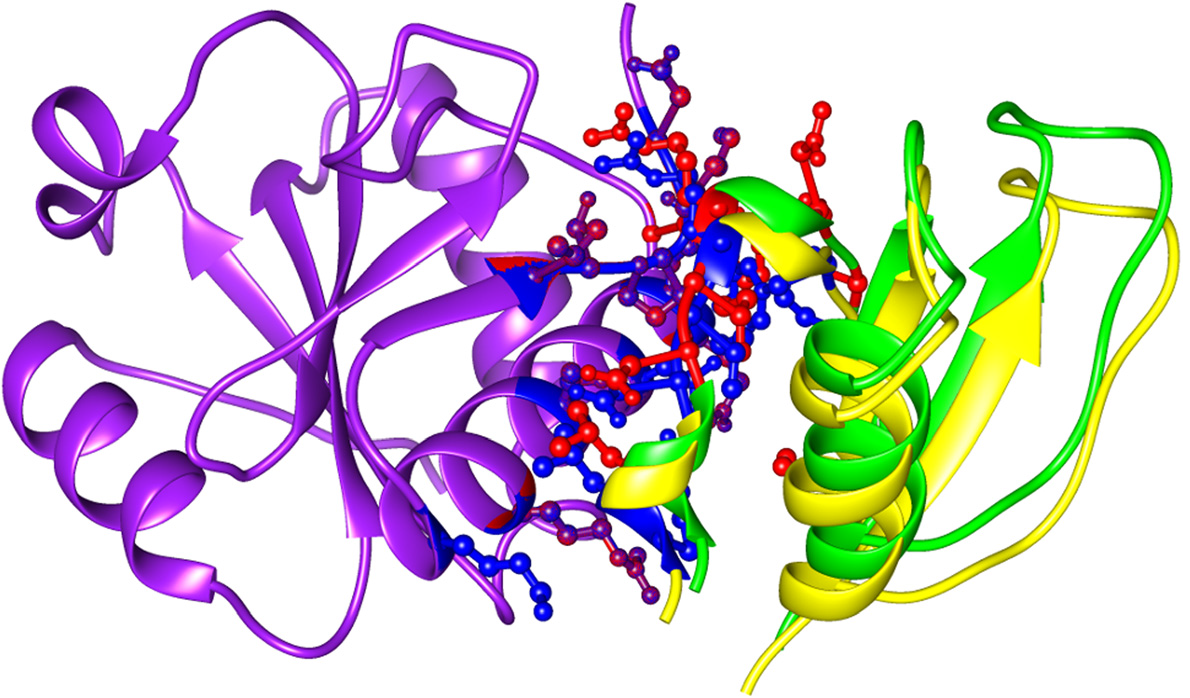
\includegraphics[width=0.8\columnwidth]{dockscore.png}
  \caption{Visual representation of the native and computed conformations of the protein complex with PDB ID 1SYX. Image taken from~\cite{Malhotra2015}.}
  \label{fig:dockscore}
\end{figure}

It is clearly visible that even for the comparison of two conformations the traditional representation suffers from many occlusion problems and it is hard to perceive the differences between individual solutions.
When comparing more conformations, even without a detailed visualization of hot spot amino acids, the problem becomes even more apparent (see Figure~\ref{fig:problem}).

\begin{figure}[tb]
  \centering
  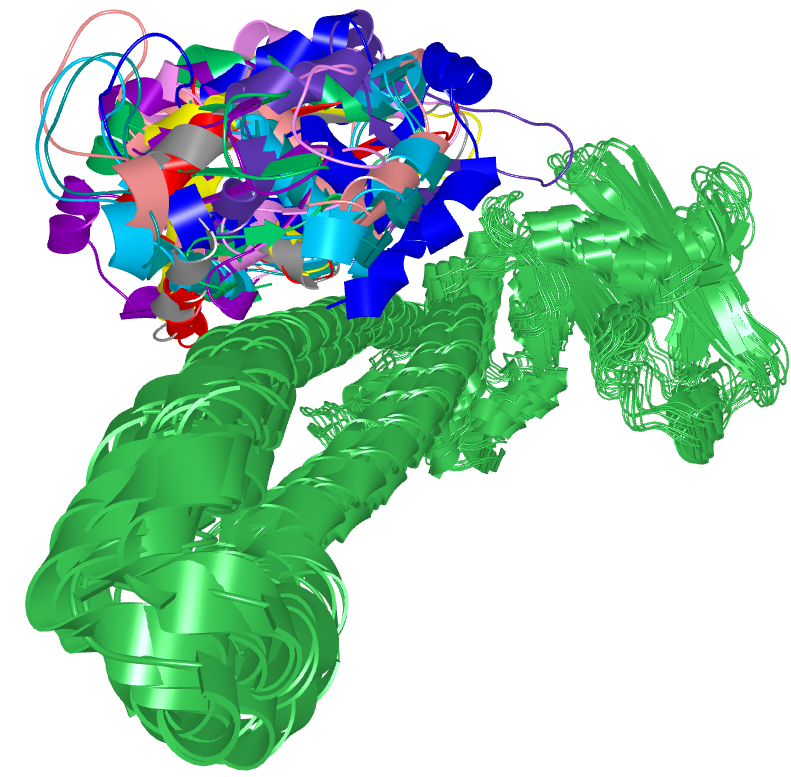
\includegraphics[width=0.7\columnwidth]{problem.png}
  \caption{Superimposition of several possible conformations between two proteins visualized using traditional cartoon rendering. The set of green protein instances corresponds to one of the interacting proteins, the colored components represent the second protein in different conformations.}
  \label{fig:problem}
\end{figure}

Therefore, in this paper we are proposing a solution to this clutter problem.
We present a set of novel methods for the visualization and comparison of individual conformations.
They aim to remove the problems of existing solutions and provide the domain experts with an intuitive and user friendly tool for an interactive exploration of protein-protein interactions provided by the computational tools.
Our solution is designed for dealing with a large number of conformations so the user is not forced to apply any of the re-ranking algorithms before using our solution. 


\section{Related Work}
In this section we review the existing techniques related to our proposed representations of protein-protein interactions.
Generally, molecular visualization represents very important and useful topic in visualization.
This was confirmed also by Kozlikova et al.~\cite{Kozlikova2015} in their survey of molecular visualization techniques.

The issue of visual representation of protein-protein interactions can be tackled from different perspectives.
One group of existing solutions focuses on the visualization of entire networks of interacting proteins.
Because of their complexity, i.e., the number of interacting proteins, the visualizations are mostly graph-based.
Jeanquartier et al.~\cite{Jeanquartier2015} presented a survey of databases enabling the visual analysis of protein networks.

The second group consists of techniques visualizing the contact zones and their interacting amino acids.
The spatial techniques have to deal with the problem of occlusion and visual clutter caused by the fact that the most interesting parts of the interacting proteins, the contact zones, are positioned close to each other (see Figure~\ref{fig:varshney}a).
In other words, without any transformation or a visual enhancement (e.g., through transparency) it is impossible to visually explore the contact zones.
Therefore, Jin et al.~\cite{Jin2014} presented the open-book view where the interacting proteins are rotated to orient the contact zones towards the camera.
The problem of the presented solution lies mainly in the missing information about the interacting amino acids and the unified coloring of the contact zones.
An alternative approach presented by Lee and Varshney~\cite{Varshney2003} computes and visualizes the intermolecular negative volume and the area of the docking site (Figure~\ref{fig:varshney}b,c).
This way the users can observe the volume between the interacting proteins without direct visualization of the contact zones themselves.
This can serve the domain experts as an interactive tool for studying possible docking conformations.

\begin{figure}[bt]
  \centering
  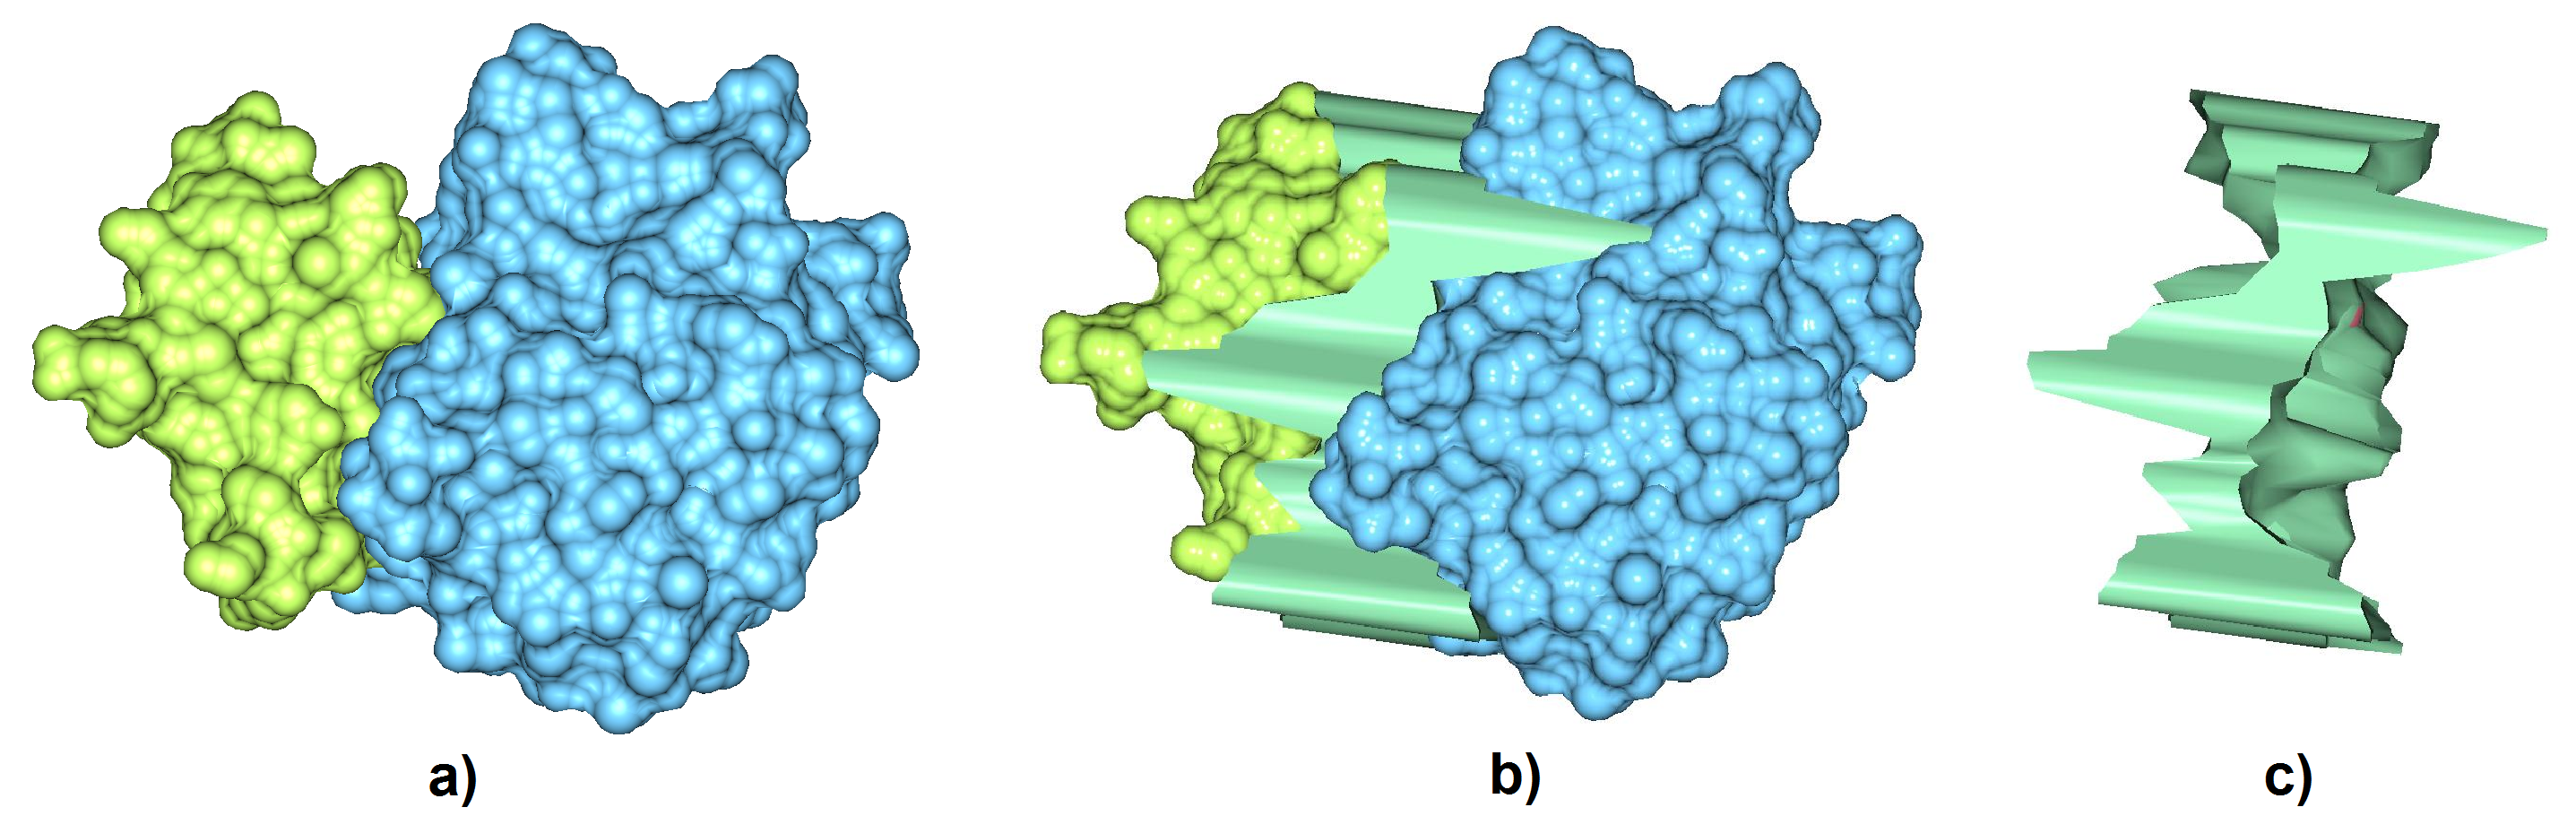
\includegraphics[width=1.0\columnwidth]{varshney.png}
  \caption{(a) Surface visualization of two interacting proteins with PDB ID 4SGB where the contact zone is not visible. (b) and (c) Visualization of the intermolecular negative surface representing the volume between the surfaces of the contact zone. Image taken from~\cite{Varshney2003}.}
  \label{fig:varshney}
\end{figure}

One of our proposed spatial visualizations adopts the idea of so called exploded views.
This technique enables to observe the parts of objects which are originally hidden.
Bruckner et al.~\cite{Bruckner2006} adopted this technique to volume data and demonstrated it on the scans of different parts of human body.

Alternative approaches to the visualization of contact zones may use abstracted 2D representations.
As an example of such an approach the schematic representation of the contact zones used in the PDBsum database~\cite{pdbsum} can be taken (see Figure~\ref{fig:pdbsum}). 
In an overview visualization each of the interacting proteins is represented by a sphere equipped with the information about the number of amino acids forming the contact zones and the number of different types of interactions between them (e.g., salt bridges, disulphide bonds, hydrogen bonds, or non-bonded contacts).
Another detailed visualization lists all contact-zone amino acids. 
The interactions are visualized by lines of different colors and thicknesses which represent the type and strength of the interaction.

\begin{figure}[bt]
  \centering
  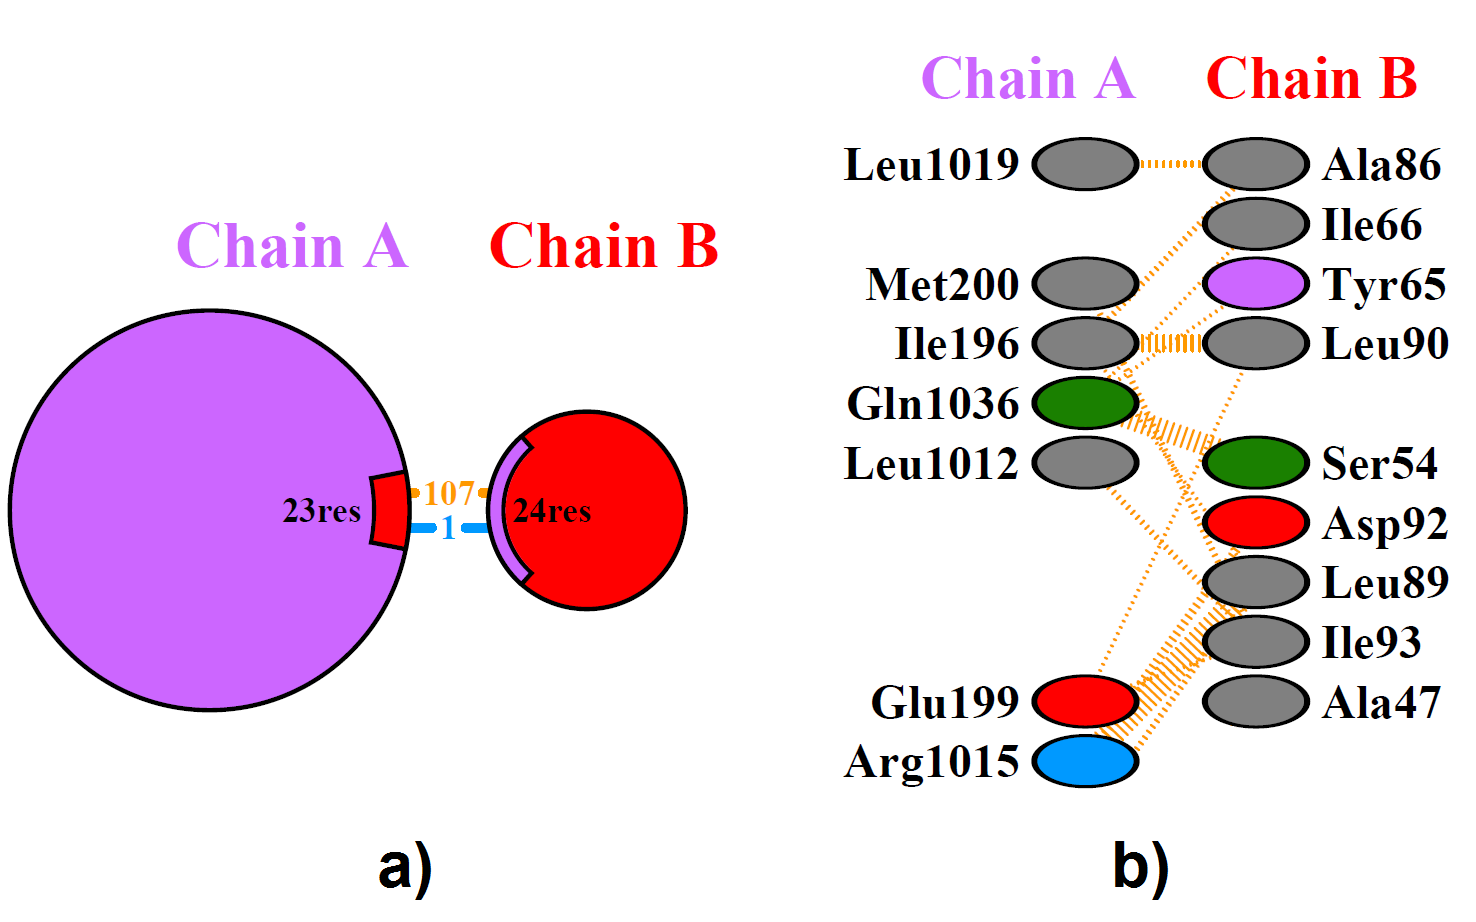
\includegraphics[width=1.0\columnwidth]{pdbsum.png}
  \caption{Two abstracted visualizations of the complex SMC3-Scc1 with PDB ID 4UX3 available in the PDBsum database. (a) Overview representation showing the number of amino acids in the contact zones and the types on interactions. (b) Part of the list of all interacting amino acids along with individual interactions and their strength. Images taken from the PDBsum database~\cite{pdbsum}.}
  \label{fig:pdbsum}
\end{figure}

Abstracted representations were already successfully applied to protein-ligand docking.
Byska et al.~\cite{Byska2015} proposed visual abstractions of tunnels serving for ligand transportation and their evolution in molecular dynamics simulations.
Their ATH and STH representations show heat maps encoding the information about tunnel openness over time.
The MoleCollar visualization shows the evolution of the shape of the narrowest part of the tunnel, its bottleneck.
The visualization contains also the information about the position and a set of physico-chemical properties of amino acids surrounding the tunnel bottleneck.

Lex et al.~\cite{Lex2012} proposed the visual analysis tool serving for exploration of large-scale heterogeneous genomics data for characterization of cancer subtypes.
They use different views onto the complex data and one of them is the method for comparison of different datasets.
The abstracted representation shows the similarities in the datasets by connecting the corresponding blocks of data. 
The thickness of the connections denotes the amount of similarities.
This representation is to some extent similar to our proposed InCo lens view but in our case it focuses more on the exploration of the interacting amino acids in individual conformations.

In another proposed method, the Conformation Matrix View, we tackle the problem of visualizing many items in a limited 2D space.
It often leads to very small space available for individual items which are then hard to perceive.
Therefore, we also had to adopt one of the interactive lens techniques which were thoroughly surveyed by Tominski et al.~\cite{Tominski2014}.


\section{Overview}
Our newly proposed visualizations tackle the problem of visual exploration of protein-protein interaction complexes.
A protein $P$ consists of a set of amino acids connected to the polypeptidic chain.
The order of these amino acids and their properties determine the spatial arrangement of the protein and influence its behavior and function.
A complex is represented by a set of mutually interacting proteins.
In our case we focus primarily on interactions between two protein structures ($P_1$ and $P_2$) forming a complex $C(P_1,P_2)$.
The spatial orientation of the complex forms a conformation.
The $i$-th conformation of complex $C(P_1,P_2)$, denoted as $CONF_i(C(P_1,P_2))$, represents one of the possible mutual orientations of this complex.
Generally, there can be $n$ possible conformations for a given complex ($1 \leq i \leq n$) and the task is to select the conformation which is the most relevant one from the biochemical point of view.
The decision is based on a combination of knowledge about the geometric arrangement of the conformation as well as other aspects, such as the physico-chemical properties of the amino acids present in the contact zone of the given conformation.

The visualization methods proposed in this paper aim to help the domain experts to visually explore a set of possible conformations detected by one of the existing computational tools and to select the most biochemically relevant ones.
Therefore, the users have to iteratively filter out those conformations which are not fulfilling specific given criteria.
To follow this workflow, summarized in Figure~\ref{fig:workflow}, we propose a set of specific visualizations. 
The input datasets consisting of dozens of conformations between two interacting proteins were computed using HADDOCK~\cite{haddock}, one of the currently most often used tools.
In the following sections we describe our newly proposed techniques in detail.

\begin{figure}[htb]
  \centering
  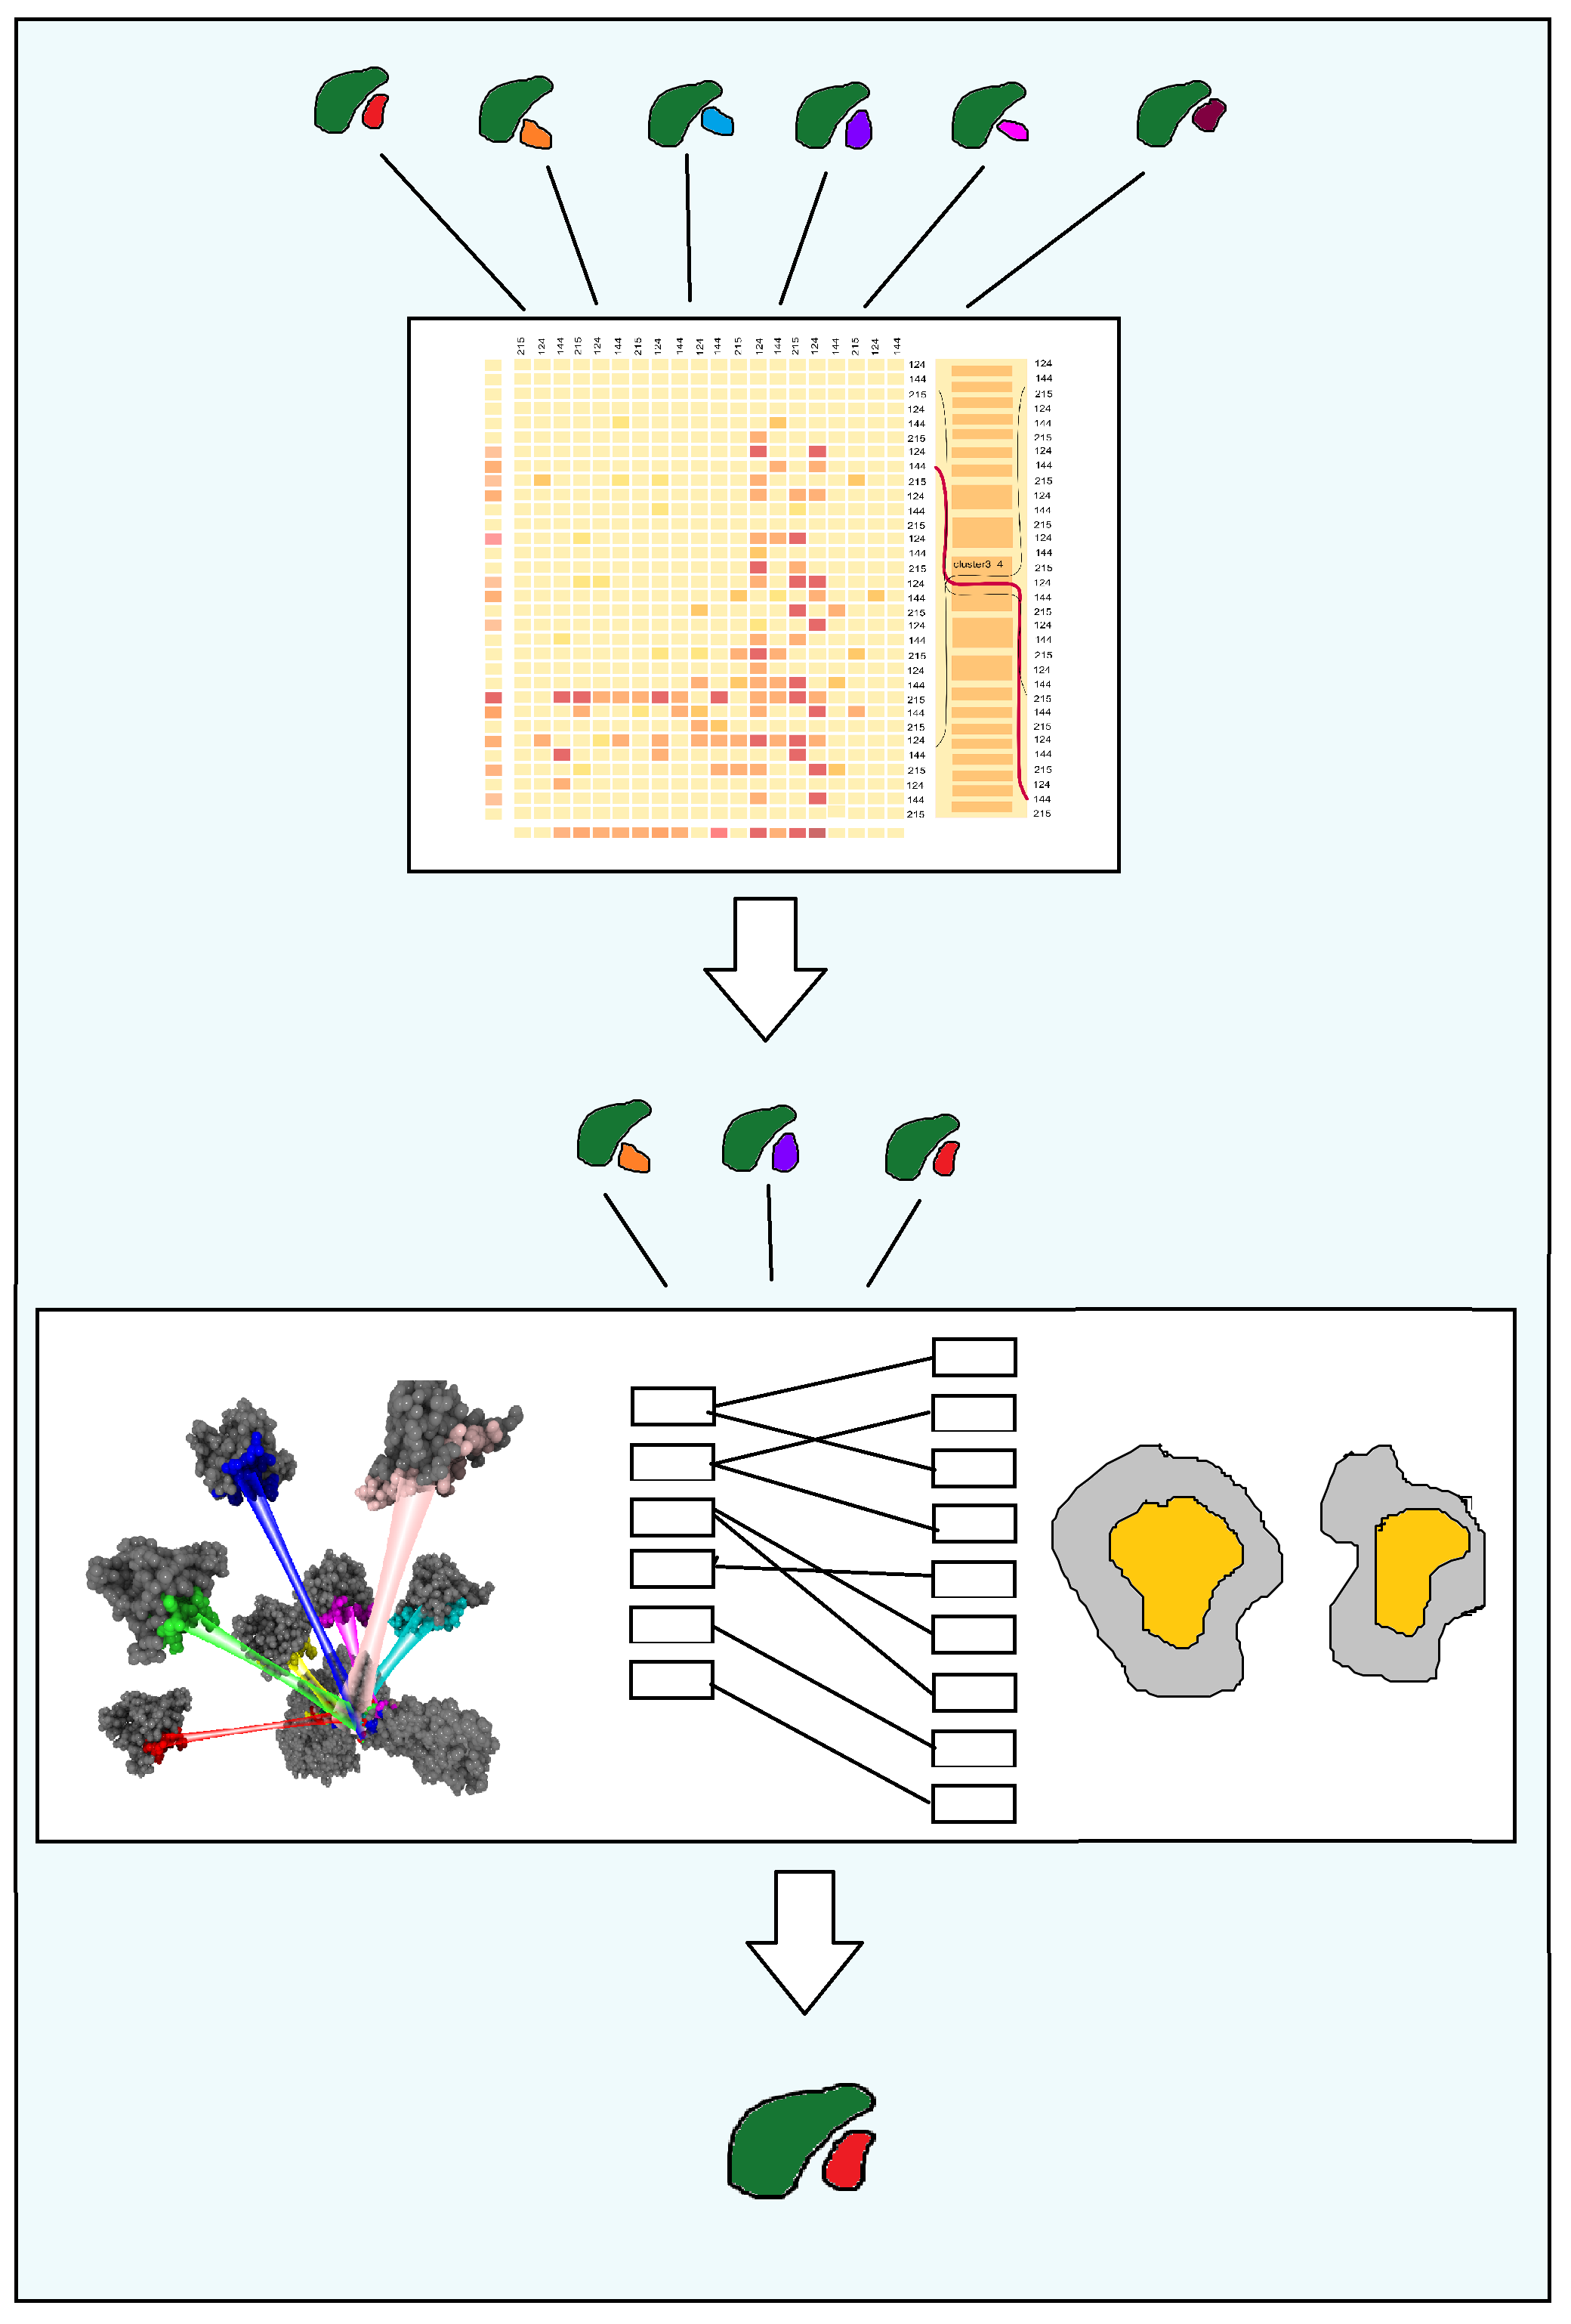
\includegraphics[width=0.98\columnwidth]{workflow.png}
  \caption{Overview of the process of exploration of the input conformations using our newly proposed methods. (a) CMV Conformation Matrix View representing an overview of all conformations. (b) InCo Lens View showing the pairs of amino acids in the interacting distance of a selected conformation. (c) CEV Conformation Exploded View enabling to explore the contact zones and their differences for a set of selected conformations. (d) COB Conformation Open-Book View animating the opening of a selected conformation. (e) CLV Conformation List View serving for detailed comparison of the constitution of the contact zones of selected conformations.}
  \label{fig:workflow}
\end{figure}

The proposed visualizations were designed to support a specific set of tasks defined by the domain experts.
They are based on the precondition that the users have some preliminary knowledge about the interacting proteins.
It mean that they are able to define a pair of amino acids from the interacting proteins that should interact.
Therefore, this information can be set as an input parameter directly to the selected computational tool.
The second option is that the users do not have such information but are aware of an already explored protein complex which can serve as a reference complex in further comparison and exploration.

Our methods were designed in order to help the domain expert to answer namely the following basic questions.
\begin{itemize}
\item Q1: Which conformations contain a selected interacting pair of amino acids?
\item Q2: What are the most frequent pairs occurring in the conformations?
\item Q3: Which pairs of amino acids are present in a given conformation?
\item Q4: Which amino acids are the closest ones in a given conformation?
\item Q5: How the contact zones are arranged and how different they are?
\item Q6: What about different properties of the amino acids in the contact zone?
\item Q7: How close the amino acids in the contact zone are?
\item Q8: How exactly the contact zone of a selected conformation looks like? How is the correspondence between its amino acids?
\item Q9: How is the difference between the sets of amino acids in the contact zones of different conformations?
\end{itemize}

Answering these questions helps the biochemist to better understand the interactions in the protein-protein complex.
The next steps of the biochemist can lead to the selection of amino acids in the contact zones which could be mutated, i.e., replaced by other amino acids.
The ultimate goal of such a mutation can be to strengthen the interactions in the contact zone or, vice versa, completely destroy the interaction between these proteins.

\section{CMV -- Conformation Matrix View}
When using a computational tool for generating possible conformations, the resulting set can be very large ($CONF_i(C(P_1,P_2))$) where $i$ spans from dozens to hundreds) and requires some preliminary filtering.
This filtering stage is based on answering questions Q1 and Q2.
To answer them, we propose a matrix-based visualization inspired by commonly used heat maps (see Figure~\ref{fig:matrixlens} left part).
The rows and columns of the conformation matrix view (CMV) correspond to interacting proteins $P_1$ and $P_2$.
Each row or column represents one amino acid present in a contact zone of some of the conformations $CONF_i(C(P_1,P_2))$. 
In other words, the rows and columns are formed only by those amino acids of the interacting proteins which are in contact in at least one conformation.
The contact between the amino acids is based on their Euclidean distance. 
Two amino acids are considered to be in contact if their distance is between 3 and 5 \AA ngstr\"{o}ms.
The color of each cell in the matrix corresponds to the number of the occurrences of the corresponding interacting amino acids in the set $S$ of all conformations, $S = \{CONF_i(C(P_1,P_2)); 1 \leq i \leq n\}$. 
In other words, the colored lists of amino acids can be perceived as histograms encoding the number of their occurrences.
The intense red color represents pairs of amino acids which are interacting in most of the conformations.
Thus, it can be anticipated that they play a significant role in the protein-protein interaction and it is meaningful to explore them in more detail.
On the other hand, rare combinations of amino acids can be filtered out.
The matrix serves directly for filtering out those improbable solutions by interactive user-driven selection of cells of the CMV.
Moreover, the matrix allows the selection of a combination of more pairs of amino acids.
This is useful if the user wants to further explore only those conformations which contain the interactions between amino acids $A$, $B$ and/or simultaneously also $C$, $D$. 

\begin{figure}[bt]
  \centering
  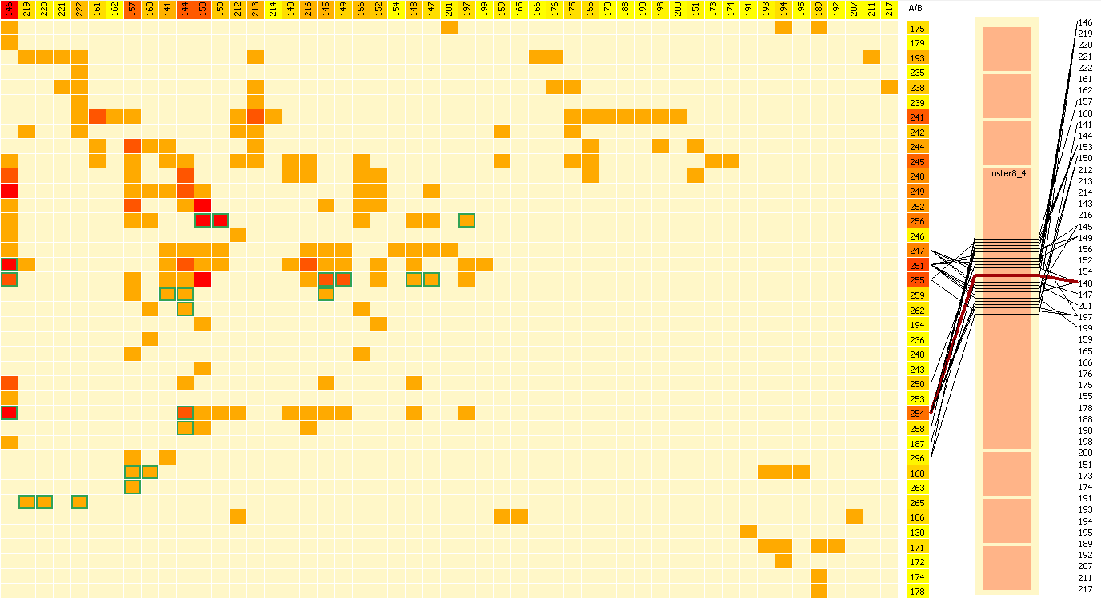
\includegraphics[width=1.0\columnwidth]{matrixlens.png}
  \caption{(a) CMV showing the aggregated information about the presence of mutually interacting amino acids in all conformations. It is interactively linked with (b) the lens view presenting more detailed information about individual conformations and their interacting amino acids. \textcolor{red}{TODO change image}}
  \label{fig:matrixlens}
\end{figure}

The rows and columns in the matrix can be also sorted according to the frequency of occurrence of the amino acids in the conformations. 
This results in the concentration of more frequent pairs of amino acids in the top left corner of the matrix (see Figure~\ref{fig:sort}).

\begin{figure}[bt]
  \centering
  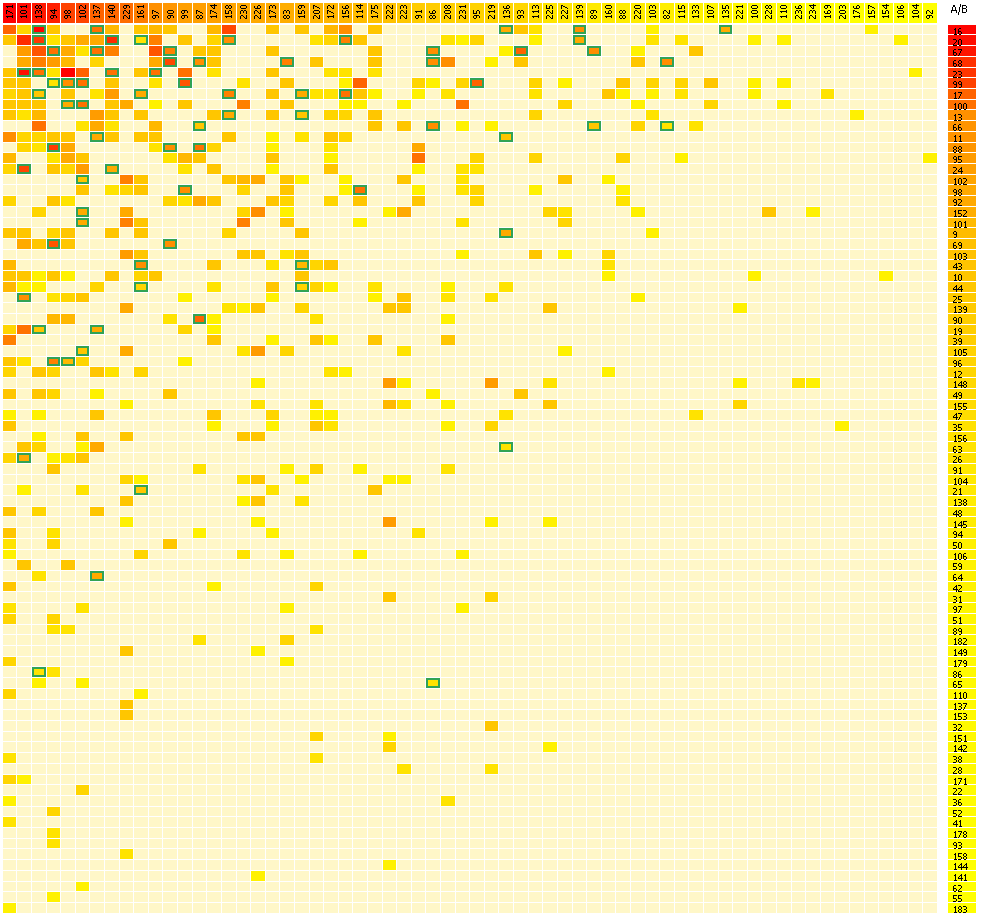
\includegraphics[width=0.8\columnwidth]{sort.png}
  \caption{Matrix view sorted according to the frequency of occurrence of the amino acids in all conformations. Green borders of some matrix cells represent the pairs which are present in some of the conformations (selected in the lens view). Selected cells are marked with a cross. Table lens technique enables to enlarge a selected cell.}
  \label{fig:sort}
\end{figure}

One of the biggest advantages of the matrix view is its independence on the size of the input set of possible conformations.
The number of rows and columns is limited by the size of interacting proteins, so in the worst case it can correspond to the total number of amino acids of these proteins.
However, usually the number of amino acids in the contact zones is very limited -- for medium-size proteins there can be approximately from 10 to 20 amino acids.
So the number of rows and columns is much smaller than this upper limit.
Then, each conformation of the input dataset increases the counters represented by the color in the matrix rectangles.
Therefore, the only parameter influencing the size of the matrix is the size of the interacting proteins.
For large proteins the rectangles of the matrix can be too small.
In such situations, the users can use the table lens technique introduced by Rao and Card~\cite{Rao1994} applied to both rows and columns of the matrix.

The matrix view is interactively linked with another newly proposed visualization, lens view, positioned directly next to the matrix (Figure~\ref{fig:matrixlens} right part). 

\section{InCo Lens View}
InCo (Interaction Contact) lens accompanying the matrix view provides the users with more detailed information about individual conformations, thus answering questions Q3 and Q4.
In the CMV the information about all conformations is merged in order to give an overview of the interacting amino acids concerning the entire dataset.
Therefore, the constitution of individual conformations, yet very important in the filtering stage, is omitted.
InCo lens view complements the CMV and presents the content of the contact zones of individual conformations in a highly abstracted way (see Figure~\ref{fig:inco}).

\begin{figure}[bt]
  \centering
  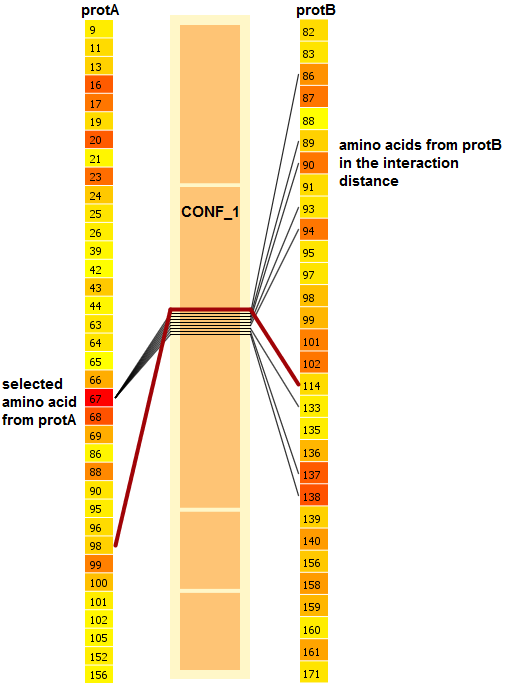
\includegraphics[width=0.8\columnwidth]{inco.png}
  \caption{InCo lens view enabling to explore the interacting amino acids in the contact zone of a selected conformation.}
  \label{fig:inco}
\end{figure}

The input conformations are coming from the filtering stage performed using the CMV.
The task is to iteratively search through this list of conformations.
So we assume the list is displayed on a scrollable wheel which forms the central part of the lens view. 
So the user can scroll the view with the mouse wheel and explore individual conformations.
The central part consists of rectangles representing individual conformations of a subset of $S$ where the rectangle in the middle corresponding to a conformation in focus gets the largest screen space.
The currently investigated conformation in the middle contains the identifier of the conformation.

The InCo view is further equipped with two lists of amino acids positioned on the left and right side of the central part.
These lists are the same as in the case of CMV, i.e., they contain all amino acids present at least in one contact zone from $S$.
The amino acids are again colored according to the frequency of their occurrence within $S$.

By default each conformation in focus contains one polyline connecting two amino acids from the contact zone which are in the closest distance from all its possible pairs of amino acids.
Furthermore, also other possible connections can be added to the InCo view.
The user can hover the mouse over the lists of amino acids on the left and right side and the corresponding connection lines for a given amino acid are appearing.
By clicking on the rectangle representing the given amino acid the connection lines remain in the view (see black polylines in Figure~\ref{fig:inco}).

The lens view is highly interactive and closely linked with the matrix view.
The pairs of amino acids forming the conformation in focus can be highlighted in the matrix view (green borders of rectangles in Figure~\ref{fig:sort}) so the user can immediately see the number of conformations in which these pairs are present as well.
Vice versa, by interacting with the matrix view and selecting given cells, the lens view can be automatically filtered and shows only those conformations which satisfy the filtering condition defined in the matrix view.

By combining the matrix and lens views, the domain expert can inspect the large input set of conformations and filter out those not satisfying the conditions derived from the preliminary knowledge about the interacting proteins.
Selected conformations can be further processed by the following visualization methods.

\section{CEV -- Conformation Exploded View}
The biochemists are already well accustomed with the manipulation of molecules in a three-dimensional environment, thus this space has to be an integral part of the workflow.
Moreover, the three-dimensional space helps to find answers for questions Q5-Q7 related to the appearance of the contact zone of selected conformations.
However, as already stated, exploring and comparing many structures in 3D at once suffers from problems with high overlaps, occlusion, and visual clutter. 
So the traditionally used representations are not sufficient (as indicated in Figures~\ref{fig:dockscore} and~\ref{fig:problem}).
To overcome these limitations, we use the technique of so called exploded views which enlarges the distance between the interacting proteins (see Figure~\ref{fig:exploded}). 

\begin{figure}[bt]
  \centering
  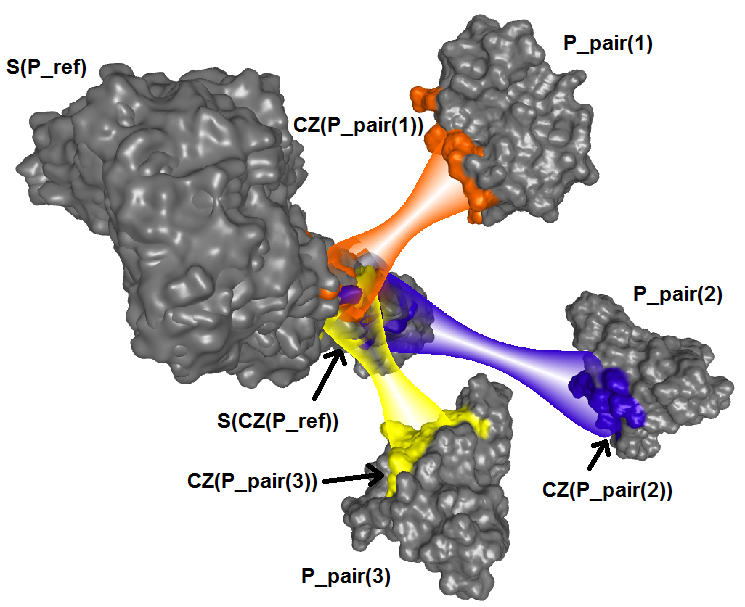
\includegraphics[width=1.0\columnwidth]{exploded.png}
  \caption{Exploded view showing the interaction between the reference protein and its paired proteins. Proteins are represented by their surface and the contact zones are colored.}
  \label{fig:exploded}
\end{figure}

To describe the principle of this technique in detail we need to introduce the following notation.
Lets assume that a conformation $CONF_i(C(P_1,P_2))$ contains a contact zone $CZ(P_1,P_2)$ of the complex $C(P_1,P_2)$.
This contact zone consists of two subsets of amino acids, each coming from one of the interacting proteins.
Lets mark as $CZ(P_1)$ and $CZ(P_2)$ the part of the contact zone belonging to protein $P_1$, $P_2$ respectively.
One of the $P_1$ and $P_2$ proteins has to be marked as a \textbf{reference protein} $P_{ref}$.
This can be done automatically (by setting the first loaded protein as the reference one) or the user can select which of the loaded proteins should be the reference one.
The set of reference proteins is then marked as $S(P_{ref})$.
Then the second protein from $C(P_1,P_2)$ is automatically marked as a \textbf{paired protein} $P_{pair}$ and the set of these protein is marked as $S(P_{pair})$.

Now we have the sufficient terminology to describe the main principle of the CEV.
First all the $S(P_{ref})$ reference proteins taken from the conformations selected by CMV and InCo views are aligned using a Combinatorial Extensions structural alignment algorithm~\cite{Shindyalov1998} (see the green protein in Figure~\ref{fig:problem}).
The set $S(P_{pair})$ interacting with the $S(P_{ref})$ is positioned around the aligned $S(P_{ref})$.
As it is expected that the set of conformations selected in the previous stage contains more than one conformation, the proteins from $S(P_{pair})$ are overlapping significantly.
Therefore, by increasing the distance between the proteins from $S(P_{ref})$ and $S(P_{pair})$ using exploded views can remove this issue.

To ensure that the paired proteins in the exploded view will not collide with each other, our algorithm calculates the spatial position of proteins from $S(P_{pair})$ based on their bounding boxes.
For each pair of interacting proteins, the vector between $CZ(P_{ref})$ and $CZ(P_{pair})$ is computed. 
$P_{pair}$ is then shifted along this vector from $P_{ref}$ by a user-defined value. 
This can lead to mutual collisions between the shifted $P_{pair}$ proteins.
Thus, the "reshuffling" of the $P_{pair}$ proteins has to be applied to avoid these collisions. 
All $P_{pair}$ proteins are put into a queue.
For each $P_{pair}$ we detect collisions with all proteins remaining in the queue.
The collision detection computation is based on the spherical bounding boxes of the proteins.
If a collision is detected, we compute the $shift_{unprocessed}$ vector for $P_{pair}$ as an averaged sum of vectors between $P_{pair}$ and all colliding proteins.
Then we compute the $shift_{processed}$ vector for $P_{pair}$ shifted by the $shift_{unprocessed}$ vector in the same way for collisions with already processed proteins (which are not in the queue).
The two shift vectors are then averaged and give the final $shift$ vector for $P_{pair}$, which is moved to its new non-colliding position.
To avoid deadlocks, the whole reshuffling process is repeated until no collisions are detected.
But the maximal number of repetitions corresponds to the number of $P_{pair}$ proteins (i.e., the number of processed conformations).

For each $P_{ref}$ and its counterpart protein $P_{pair}$ the CEV maintains the information about their interaction.
This is important because when more conformations are exploded at once the CEV contains many $P_{pair}$ proteins scattered around the aligned $P_{ref}$ proteins and the pairing information is completely lost.
Therefore, we display the connection between corresponding $P_{ref}$ and $P_{pair}$ as a tube connecting the centers of parts $CZ(P_{ref})$ and $CZ(P_{pair})$ of the contact zone.
The radius of the tube at each point of the segment is modulated by its distance to the segment endpoints.
The opacity of the tube is modulated in screen space, depending on the distance to the segment centerline.

Figures~\ref{fig:case2} and~\ref{fig:case3} presenting the set of five conformations before and after using the CEV show that it removed not only the problem of overlapping paired proteins but also enabled the user to see the contact zones which were in the original position of interacting proteins hidden between them.
However, this solution does not solve the problem that the contact zones are still facing each other so the user has to manipulate with the camera to observe $CZ(P_{ref})$ or $CZ(P_{pair})$ from a perpendicular view. 
But even such manipulation does not enable to see $CZ(P_{ref})$ and $CZ(P_{pair})$ at once (one of them is always located on the opposite side of the camera).
This problem is solved by the Conformation Open-Book view presented in the following section.

\section{CoOp -- Conformation Open-Book View}
As stated above, the CEV suffers from the problem of intuitive navigation through the space to observe the $CZ(P_{ref})$ and $CZ(P_{pair})$ parts of the contact zones in detail and at once.
The CoOp view is designed specifically to answer questions similar to Q8 which are dealing with the problem of detailed exploration of a selected contact zone $CZ(P_1,P_2)$ of the complex $C(P_1,P_2)$.
This involves the presentation of the information about different properties of individual amino acids forming the contact zone and their pairing.

The CoOp view is activated when the user selects one of the conformations from the exploded view. 
The selection is performed by clicking on the connection tube of the desired conformation $CONF_i(C(P_{ref},P_{pair}))$ in the CEV.
The other conformations present in the CEV are automatically hidden and an animated transition of the opening of the $CONF_i(C(P_{ref},P_{pair}))$ is launched.
Within the animation in which the $P_{ref}$ and $P_{pair}$ proteins are rotated and translated so that they are positioned next to each other and $CZ(P_{ref})$ and $CZ(P_{pair})$ parts of the contact zone are facing towards the observer (see Figure~\ref{fig:book}). 

The algorithm works as follows.
First we compute the center of mass of proteins $P_{ref}$ and $P_{pair}$, lets denote them $A$ and $B$.
Then we find also the center of mass of both $CZ(P_{ref})$ and $CZ(P_{pair})$, lets denote them $A_{CZ}$ and $B_{CZ}$.
It is worth to mention that the vector between $A_{CZ}$ and $B_{CZ}$ in fact corresponds to the centerline of the tube connecting $P_{ref}$ and $P_{pair}$ in the CEV.
Then we compute the normal vectors for both $CZ(P_{ref})$ and $CZ(P_{pair})$ as $N_A = B_{CZ} - A_{CZ}$ and $N_B = A_{CZ} - B_{CZ}$.
In the following step the vectors heading from $A_{CZ}$ and $B_{CZ}$ to the camera position $CAM$ have to be computed.
We will get them as $CAM_A = A_{CZ} - CAM$ and $CAM_B = B_{CZ} - CAM$.
The normal and the camera vectors are then used for the computation of the rotation angle which is then applied to $P_{ref}$ and $P_{pair}$.
Before the rotation itself, for each protein it is necessary to find the rotation axis.
This axis is perpendicular to the normal and camera vectors and is computed as their cross product $cross(N_A,CAM_A)$, $cross(N_B,CAM_B)$ respectively.
As the centers of rotation are selected $A$ and $B$ and $P_{ref}$ and $P_{pair}$ are rotated around the computed rotation axes and rotation angles.

To maintain the information about the pairing of amino acids, the user can visualize also individual connections by simple lines (see Figure~\ref{fig:book}).

\begin{figure}[bt]
  \centering
  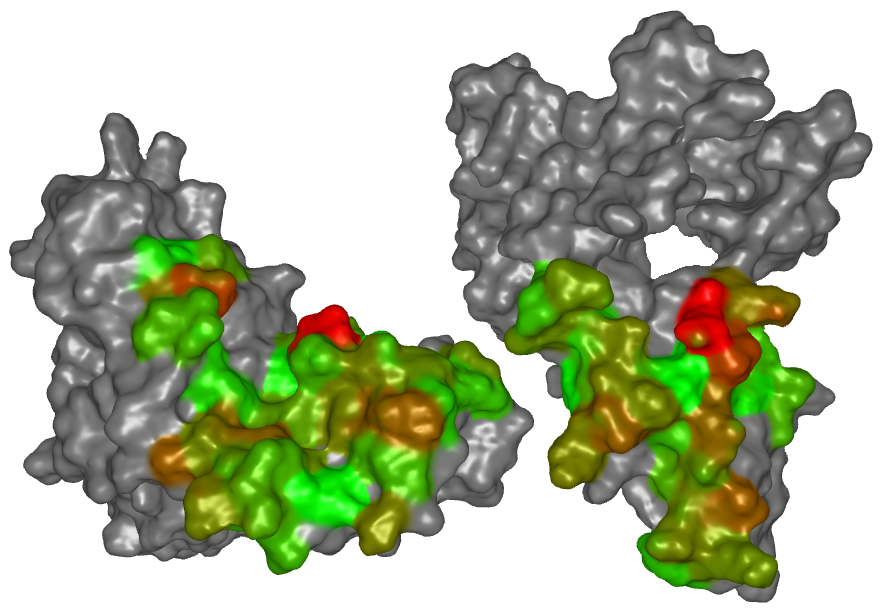
\includegraphics[width=0.8\columnwidth]{book.png}
  \caption{Conformation Open-Book View enabling to explore the contact zones between the interacting proteins simultaneously. The surface of the contact zones can be color-coded according to different criteria -- here the color represents the distance between the pairs of amino acids. \textcolor{red}{TODO change image, programming still in progress}}
  \label{fig:book}
\end{figure}

The contact zones represented by their surface can be color-coded according to different criteria.
The color can correspond to the mutual distance between the amino acids -- the closest amino acids have a different color than the most distant ones.
Color can also represent different physico-chemical properties of the amino acids or their atoms, such as hydrophobicity or partial charges.
To inform the users about the types and identifiers of individual amino acids, the surfaces can be augmented with labels bearing this information.

In both the exploded view and the open-book view the protein can be represented also by other traditionally used visualization methods, such as cartoon, spheres, balls\&sticks, sticks, etc.
Moreover, these methods can be combined so, for example, the proteins can be represented by cartoon method and the amino acids in the contact zones can be visualized using sticks representation to see their spatial orientation.% (see Figure~\ref{fig:contact}).

The combination of the CEV and CoOp view is very useful for exploration of individual conformations.
If the task is to compare individual conformations with respect to the pairs of interacting amino acids, a further drill-down is necessary.
Therefore, we propose in the next section another abstracted view serving mainly for the comparison of the paired amino acids in individual contact zones.

\section{CoLi -- Conformation List View}
The CoLi view helps to answer questions related to the comparison of the contact zones on the level of individual amino acids, such as in Q9.
It consists of two sets of amino acids in the contact zones, each set coming from one interacting protein (see Figure~\ref{fig:list}).
The left part contains all amino acids coming by default from the $P_{ref}$ protein, the right part is formed by their counterparts in the $P_{pair}$ protein.
However, the order of proteins in the list view can be changed.
The order depends on the current task -- if we want to compare the constitution of $CZ(P_{ref})$ or $CZ(P_{pair})$ in the given conformations.
The view contains all possible connections (wrt. the distance) between amino acids from both contact zones.
To avoid cross sections of lines representing the connections, some amino acids on the right side are repeated -- one occurrence for each amino acid in the reference protein within a distance of 5 \AA. 
This solution was adopted because of many line crossings in the solution without the repetition of the amino acids.

\begin{figure}[bt]
  \centering
  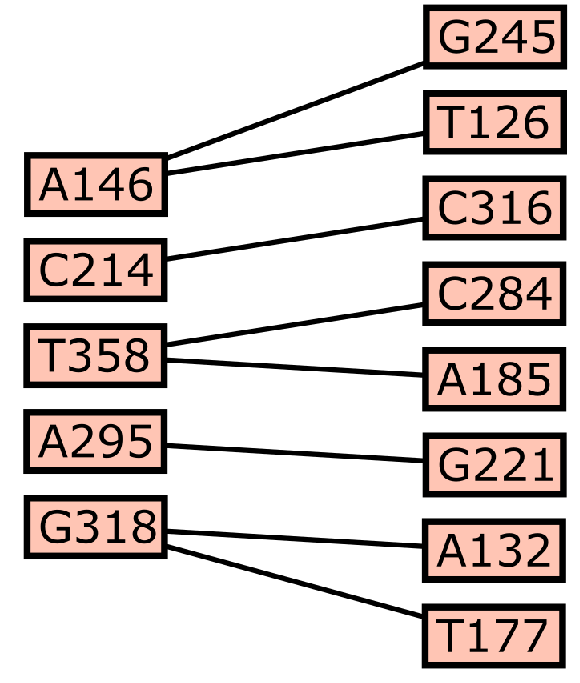
\includegraphics[width=0.7\columnwidth]{list.png}
  \caption{Compact list view (left) showing all pairs of amino acids from interacting proteins which are in interaction distance. Compare list view (right) serves better for comparison of different conformations. It preserves the blank space for amino acids which are in the contact zone in some of the conformations but not in this particular one.}
  \label{fig:list}
\end{figure}

For each conformation one list view is created and all list views are juxtapositioned so the user can see and visually compare the constitution of the contact zones of all selected conformations.
The horizontal ordering of the views can be user defined.
The user can interact with this representation by changing the properties of the amino acids mapped onto their corresponding rectangles (same properties as those mapped onto the surface in the 3D views) and sort the left part of the list according to these properties (see Figure~\ref{fig:sorting}).
Moreover, by clicking on individual rectangles representing amino acids, the corresponding amino acids are selected in the 3D view as well.

\begin{figure}[bt]
  \centering
  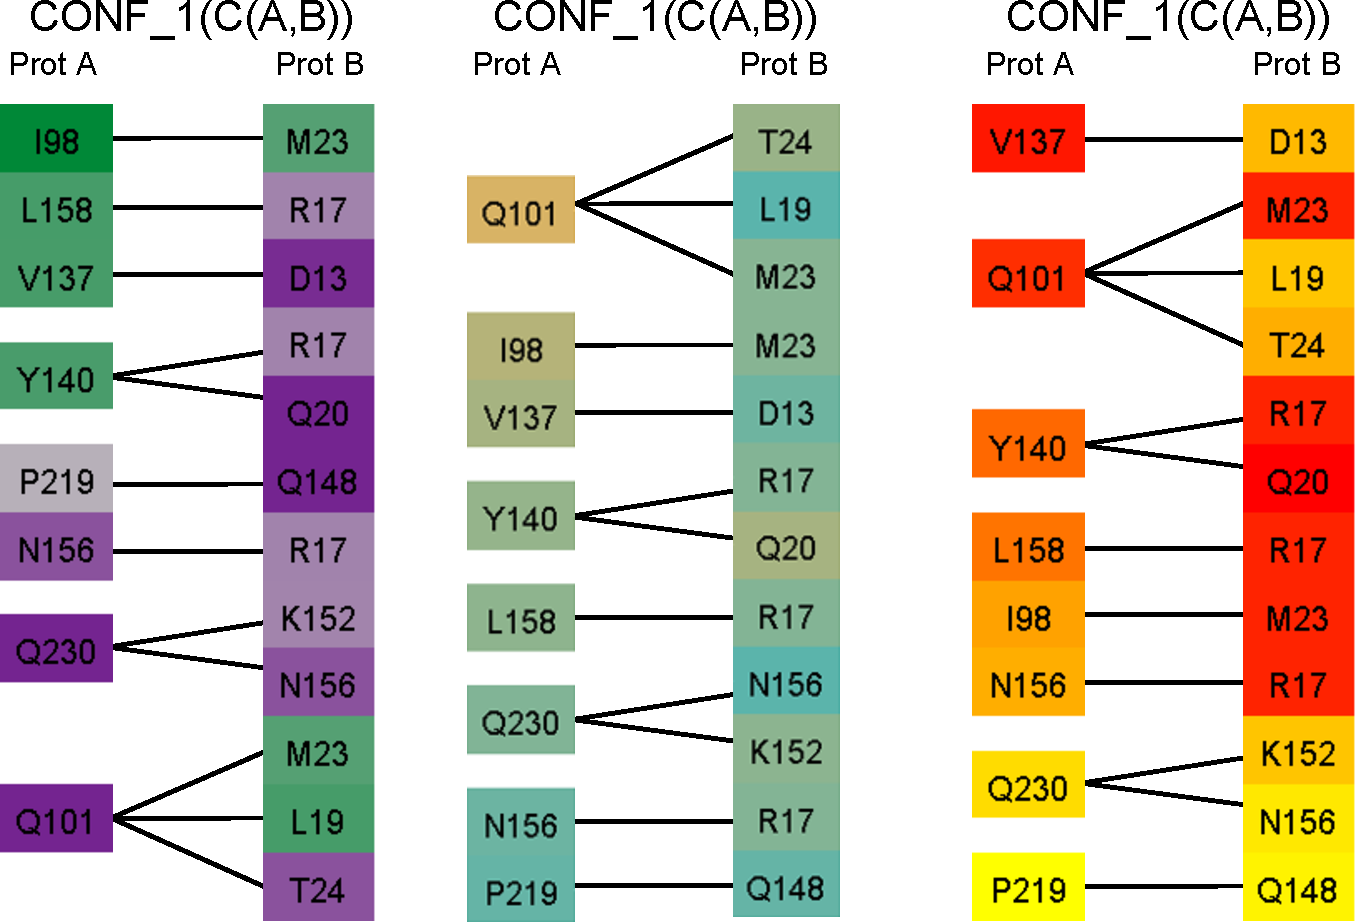
\includegraphics[width=1.0\columnwidth]{sorting.pdf}
  \caption{Sorting of the list view according to different properties of amino acids -- (a) hydrophobicity, (b) mutual distance, (c) frequency of occurrence.}
  \label{fig:sorting}
\end{figure}

The main principle of the algorithm building the CoLi is the following.
For all conformations which should be visualized in CoLi and all amino acids in their contact zones we find the closest interacting pair of amino acids (same pair as that one represented by the default polyline in the InCo view).
Then the list of amino acids present in all $CZ(P_{ref})$ of selected conformations is created.
Now, for each conformation, we take the list of the closest amino acids detected in the first step, sort them according to a selected criterion, and plot them to CoLi.

The user can select between two modes -- the compact list view and the compare list view.
The difference lies in the positioning of the amino acids in the left part of the CoLi which is always that one used for comparison because here the list of amino acids is always sorted in the same way. 
In the compare mode, each amino acid has its fixed position and if this amino acid is not present in the contact zone for some conformation, it is depicted as a white rectangle with the name of this missing amino acid (see Figure~\ref{fig:list} right).
Because the comparison and sorting is performed only in the left part of CoLi, these white rectangles are occurring only in this part.
The compact mode ignores the missing amino acids and arranges the amino acids to the most compact form to save space (Figure~\ref{fig:list} left).


\section{User Interaction}
Some of the interaction possibilities were already described along with the explanation of individual proposed visualizations.
All proposed visualizations are interactively linked to support the workflow of the biochemists as much as possible.
This means that by the selection of cells in the CMV the user automatically filters out those conformations which do not fulfill the filtering criteria and these conformations are further omitted from the other views as well.
Of course, the user can at anytime return to the beginning of the process. 
By iterative refining of the filtering using the matrix and lens views the set of conformations can be further narrowed.
Another possible scenario is that the user finds out that some of the promising conformations were filtered out at the beginning.
Such conformations can be then included back into the exploration process.

\section{Demonstration and Results}
All presented techniques were designed in tight cooperation with the domain experts from the field of functional genomics and proteomics.
Their current main research focus is on structure maintenance of chromosome (SMC) complexes~\cite{Hudson2011,Guerineau2012,Palecek2015}. 
The SMC complexes are key players in the chromatin organization where they ensure the proper condensation of chromosomes. 
The researchers analyze the architecture and function of such complexes using a variety of experimental approaches. 
Their goal is to uncover the way the subunits of these complexes interact with each other and execute unique function(s) of these complexes. 
Therefore, a visual representation of such information is highly beneficial because it helps to reveal the spatial relationships between the subunits in an intuitive way.

To demonstrate the usability of our proposed techniques, the domain experts selected an example of the human hNSE1-hNSE3 complex~\cite{Doyle2010}.
The crystal structure of this complex represents the dimer of kite proteins which is critical for function of the SMC5/6 (structure maintenance of chromosome) complex~\cite{Zabrady2016}. 
The dimerization interface of these two interacting winged-helix domains is typical for the whole kite protein superfamily~\cite{Palecek2015}.
The crystal structure was already examined in detail and the resulting conformation is already published in the PDBsum database under the PDB identifier 3NW0. 
Therefore, it can serve as a testing complex for both computational tools as well as our proposed visualizations.
In this case the domain experts provided the computational tools with the prior knowledge about one pair of interacting amino acids, Leucine with ID 97 from the $P_{ref}$ protein and Methionine with ID 23 from the $P_{pair}$ protein.
They selected the web version of the HADDOCK tool for producing the set of possible conformations. 
The tool resulted in 40 conformations.
HADDOCK internally groups the conformations into clusters, according to their similarity (defined internally by HADDOCK).
In our case we obtained 10 clusters, each containing 4 conformations.

All computed conformations were loaded to our visualization system incorporating all proposed visualizations.
From these conformations the CMV was computed which contains the frequency of occurrence of all pairs of amino acids in interaction distance within these 40 conformations.
The matrix immediately revealed one very interesting result.
Even as the user sets the input pair of amino acids, only a small portion of the resulting conformations really contains this interaction.
In our particular case, only in five conformations the Leucine 97 and Methionine 23 amino acids were within the interacting distance (less than 5 \AA ).
Of course, the conformations not fulfilling this criterion could be automatically discarded and even not integrated into the CMV.
But this is not desirable because the contact zones are formed by many interacting amino acids and the matrix showing their frequency gives the user the information that even when the selected pair is not in the interaction distance the conformation it can be still promising because of the other interacting pairs.
Moreover, the algorithm for the computation of amino acid pairs takes strictly the threshold of 5 \AA.
So when the distance is only slightly bigger, the pair is not detected.

The conformations preselected by the CMV can be further scrutinized using the InCo view.
This can further narrow the set of conformations passed to the next stage where the conformations are explored in three-dimensional space. 
In our case study the InCo view helped the biochemist to confirm the initial selection made by the CMV because in all five conformations it confirmed that the most frequent amino acids are in the interaction distance.
Thus there is a high probability that these will occur also in the contact zone of the resulting biochemically relevant conformation.

In the next step, the five conformations started to be explored in the 3D space.
The first interacting protein was selected as the reference $P_{ref}$ and all five conformations were aligned with respect to $P_{ref}$.
The $P_{pair}$ proteins were positioned around $P_{ref}$.
Figure~\ref{fig:case1} shows the situation where the five conformations are visualized using the traditional method.
Conformations are represented as surfaces and the contact zones are highlighted using different colors.
However, the most interesting parts, the contact zones, are completely hidden.

\begin{figure}[bt]
  \centering
  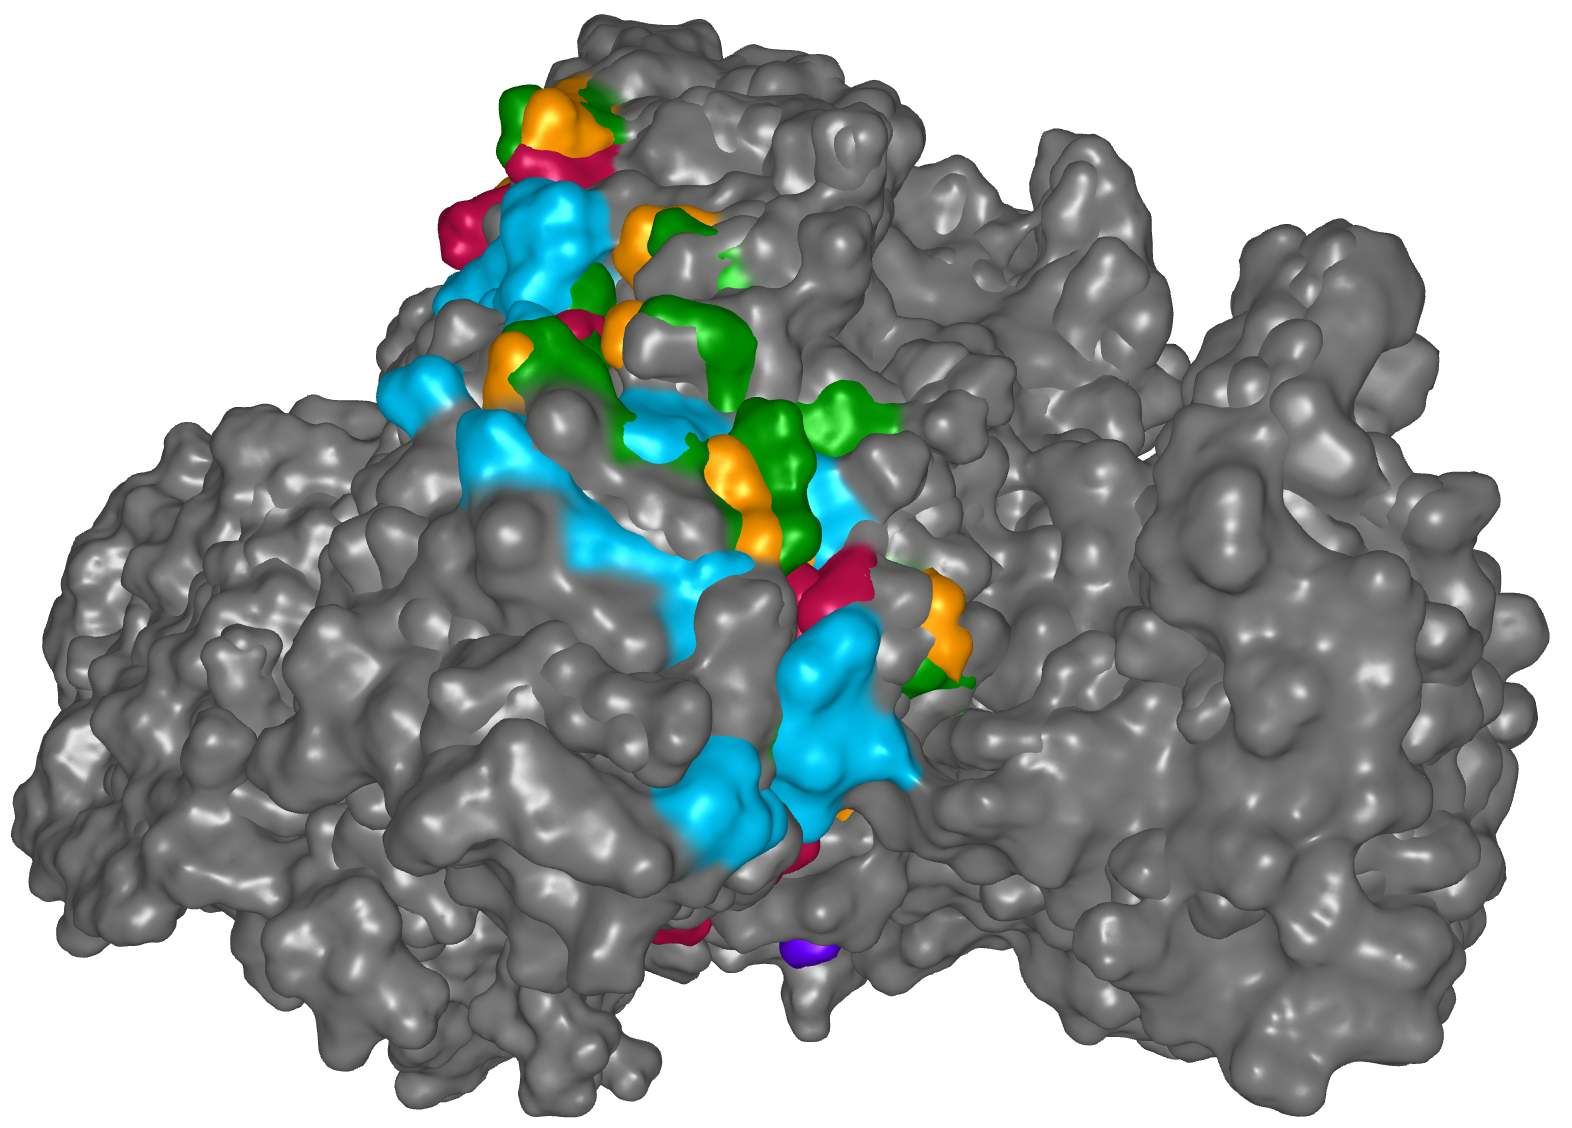
\includegraphics[width=0.7\columnwidth]{case1.png}
  \caption{Five conformations represented by surfaces with highlighted contact zones. It is clearly visible that such a representation is insufficient for the observation and comparison of the contact zones.}
  \label{fig:case1}
\end{figure}

Our exploded overcame this limitation (Figure~\ref{fig:case2}) so the individual contact zones on all $P_{pair}$ proteins are clearly visible.
Moreover, when the user is heading with the camera towards the $P_{ref}$, the differences between the positions of the contact zones in the $P_{ref}$ can be observed as well.
The connection tubes were appreciated by the domain expert because when rotating with the scene the user can be easily lost the information about the direction of the shift between the proteins.
The CEV representation gave the domain expert very interesting information about mutual positioning of individual conformations with respect to the positions of the contact zones.

\begin{figure}[bt]
  \centering
  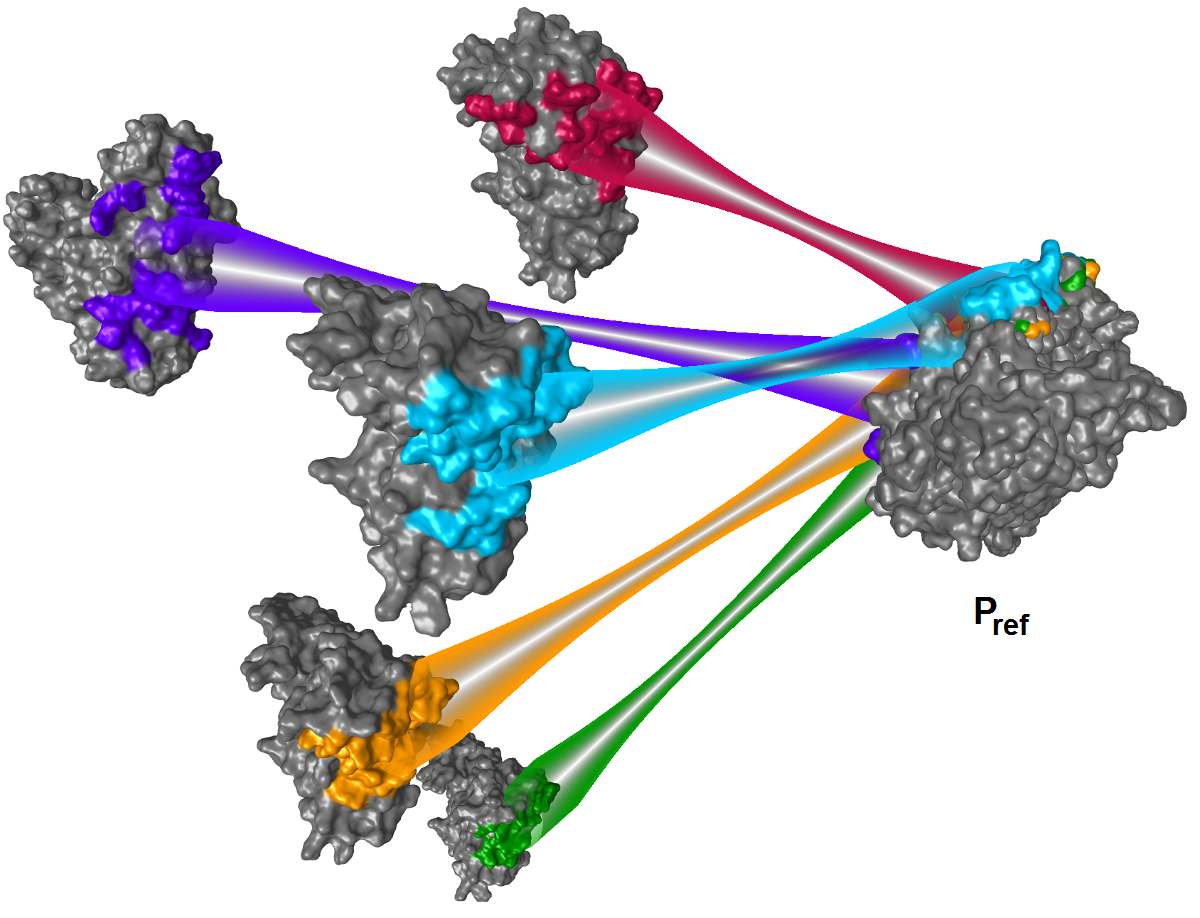
\includegraphics[width=1.0\columnwidth]{case2.png}
  \caption{Five conformations represented by the exploded view.}
  \label{fig:case2}
\end{figure}

However, the exploration has to go more deeply to the level where individual contact zones can be explored in detail.
In this case each conformation can be explored individually using the CoOp view.
By animating the opening of the contact zone the user was able to look inside the contact zone and reveal individual amino acids.
The enhancements of the CoOp view, i.e., the possibility to see the connection lines between the interacting amino acids, labeling the surface of the contact zones by the names of these amino acids, and coloring according to different criteria were highly appreciated by the domain expert.
This helped to clearly understand the constitution of the contact zone and all its properties.
After the exploration using the CoOp view the user returned to the unopened view and used the possibility to visualize the polypeptidic chains of the interacting proteins in more abstracted way using a cartoon representation. 
This allowed him to add the detailed representation of interesting pairs of amino acids selected using the CoOp view.
These pairs were subsequently visualized using a balls\&sticks method so the mutual orientation of the amino acids was visible.
%(see Figure~\ref{fig:contact}).

%\begin{figure}[bt]
%  \centering
%  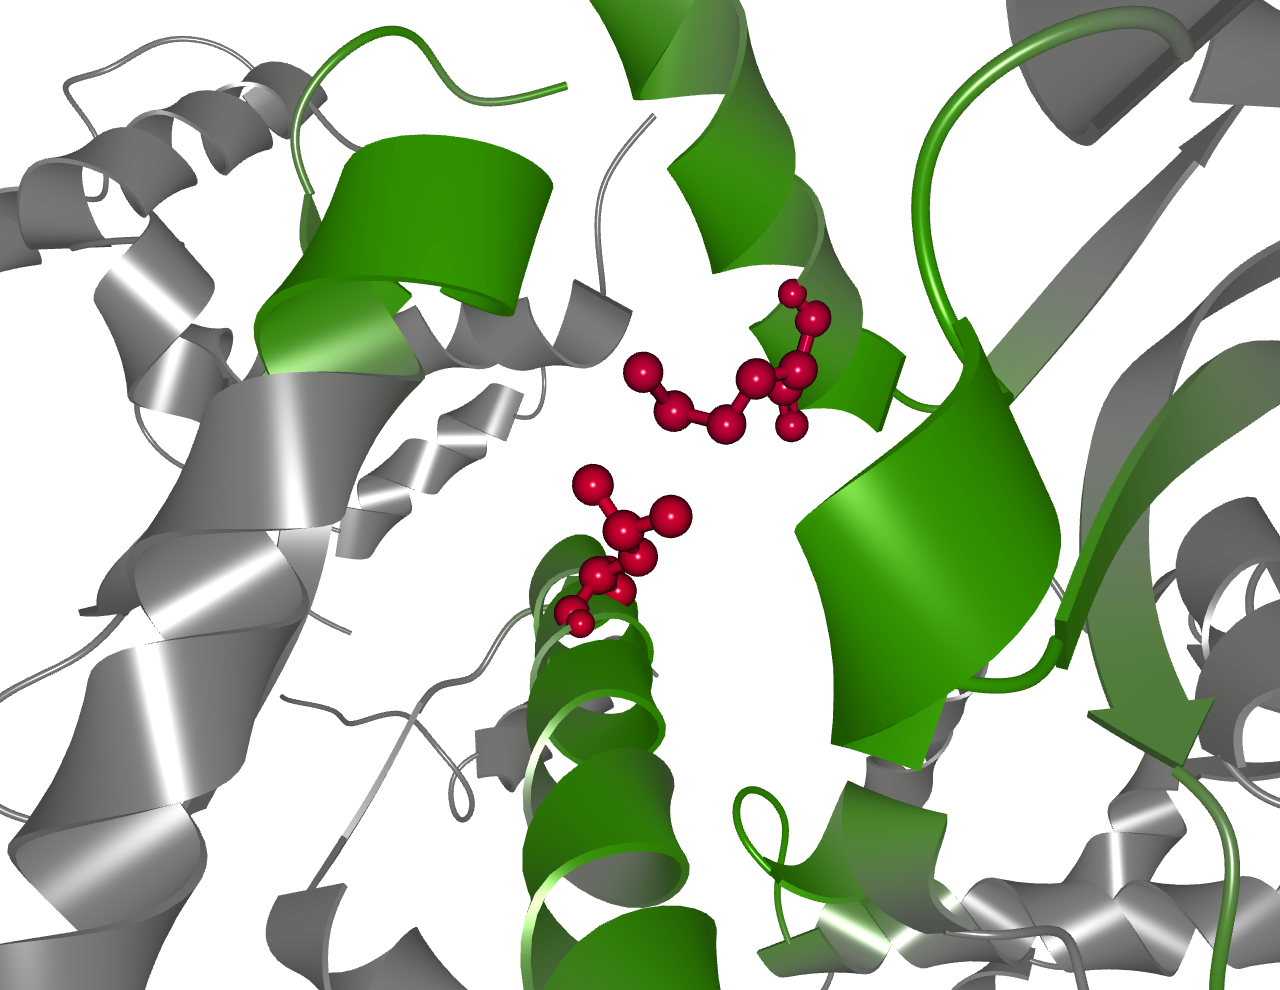
\includegraphics[width=0.8\columnwidth]{contact.png}
%  \caption{Cartoon representation of the interacting proteins where green color corresponds to the contact zone. Leucine 97 and Methionine 23 interacting amino acids are highlighted using the balls\&sticks method and the color corresponds to their hydrophobicity. \textcolor{red}{TODO change image}}
%  \label{fig:contact}
%\end{figure}

After a thorough exploration of individual conformations the user returned to the comparison stage which was hard to perform using the previous methods.
In this stage the domain expert appreciated the simplicity of the CoLi view where it is easy to compare the lists of amino acids from $P_{ref}$ or $P_{pair}$ in different conformations. 
Figure~\ref{fig:case3} shows the resulting CoLi views for our five conformations.
The left part of the views contains the list of amino acids in the contact zone of $P_{ref}$, the right part represents $P_{pair}$.
From this view it is clearly visible that the contact zone of the conformation $CONF_5(C(P_{ref},P_{pair}))$ contains much less amino acids in the $P_{ref}$ than the other conformations. 
The amino acids which are missing in this conformation but are present in the others are also detected very easily.
On the other hand, conformations $CONF_1(C(P_{ref},P_{pair}))$, and $CONF_3(C(P_{ref},P_{pair}))$ are the most similar with respect to the number and type of amino acids. 
The conformations can be compared also pairwise and the CoLi view reveals the differences in their sets of amino acids.

\begin{figure*}[bt]
  \centering
  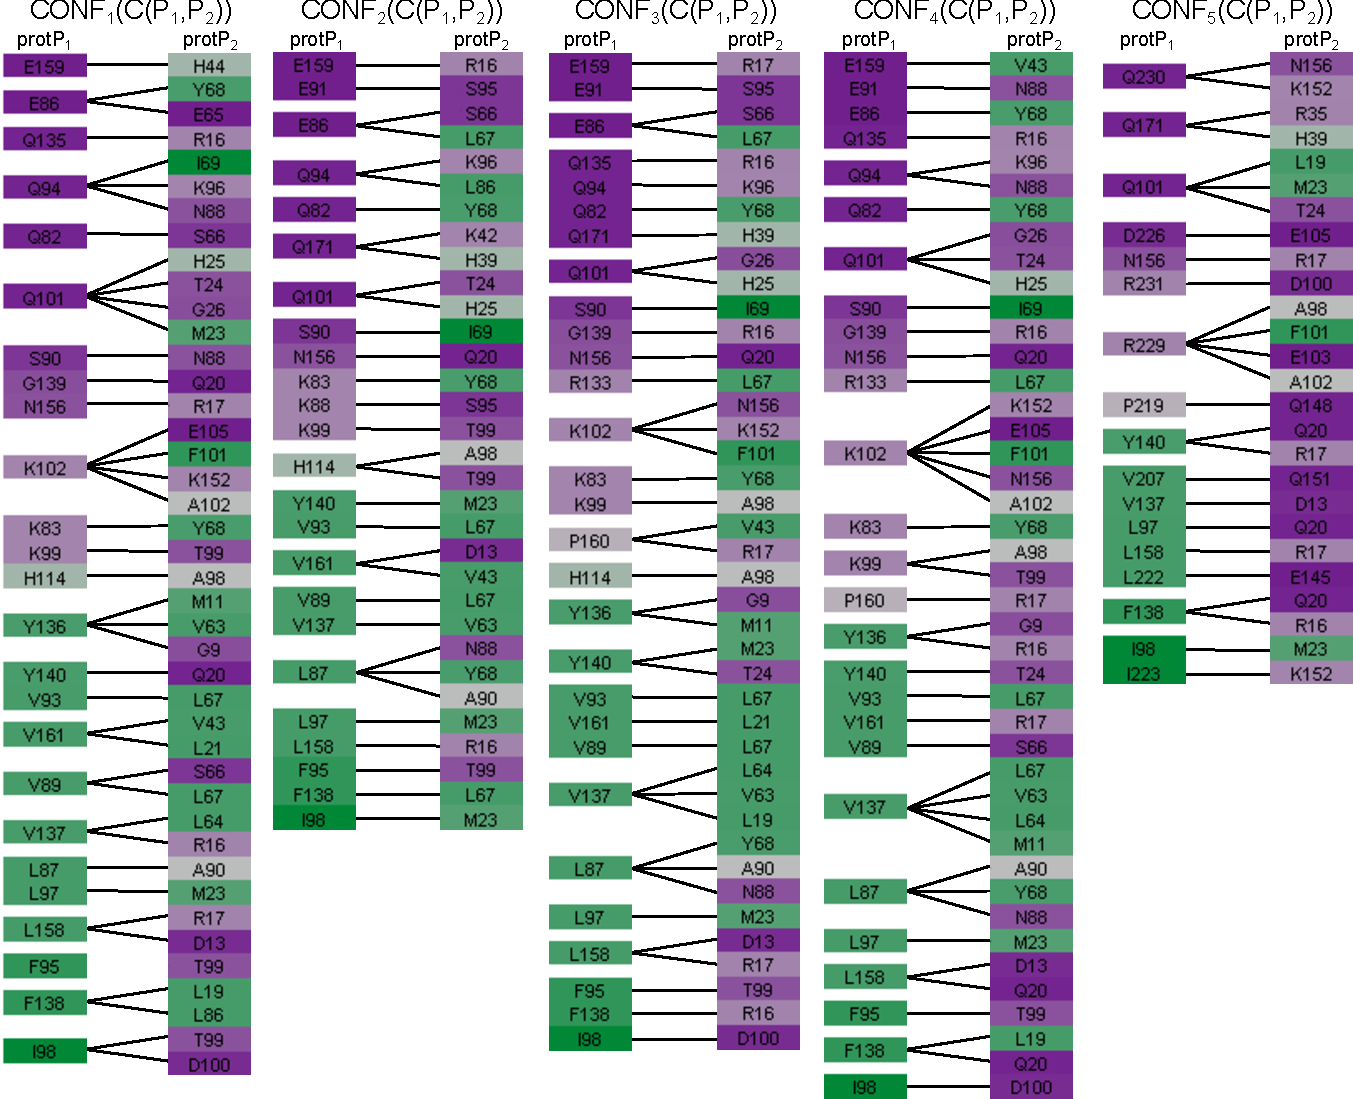
\includegraphics[width=0.9\linewidth]{case3.pdf}
  \caption{Five conformations represented by juxtapositioned CoLi views, colored and sorted according to the hydrophobicity of the amino acids.}
  \label{fig:case3}
\end{figure*}

At the end of this process the domain expert confirmed that he obtained enough relevant information to decide that the conformation $CONF_5(C(P_{ref},P_{pair}))$ is not the relevant one and the remaining, very similar, conformations is worthwhile to test in the laboratory.
He gained enough information to select possible candidate amino acids for mutation which should lead to the strengthening of the interaction within this complex.

Finally the domain expert confirmed the correctness of the selection by the comparison of the resulting conformations with the 3NW0 structure from the PDBsum database.
He confirmed that the conducted case study confirmed the usefulness of our proposed methods namely in two cases.
The first case helps to evaluate the correctness of the outputs of the existing computational tools when testing them on already know protein complex (as in our case).
By comparing the known information about the complex with the outputs of the tool the user has the idea about the relevance of the results.
In our case study we came to the conclusion that the HADDOCK results were relevant only in 10\% of all resulting conformations.
The same test was performed for the PyDock tool~\cite{pydock} and the percentage of the relevant results was even lower.
However, the conclusion about the correctness of the computational tools can be made only after performing much larger set of testing.

The second possible case where our visualizations can be highly beneficial is related to the research of newly modeled protein complexes.
The researchers are often taking the known crystal structure of a complex and are modeling its homologous structures in order to create a variant of the known complex for another organism.
These new homologous structures are very similar to the reference crystal structure but even slight differences in the structure can influence the interaction between the proteins substantially.
Therefore, the detailed exploration of these differences in crucial and here our proposed visualizations can play an important role as well.

\section{Conclusion}
In this paper we present novel visualization methods for the exploration and evaluation of biochemical relevance of large sets of conformations detected by existing computational tools.
Our proposed methods are designed to follow the workflow of the domain experts.
We described their design rationale and principles as well as the possible interactions. 
The methods were tested by the domain experts on real datasets of structure maintenance of chromosome complexes and we demonstrated the usability on one of the executed case studies.
The domain expert confirmed that our proposed solution provides him with information which was very hard or even impossible to get using the previously available methods.
He proved that using our solution their exploration process can lead to a satisfying conclusion about biochemical relevance of individual conformations much faster because it enables to iteratively filter out conformations not satisfying given conditions in individual stages of the workflow.

In the future we will focus on the extension of our proposed techniques to more complicated cases when the user has no preliminary knowledge about the protein complex.
We also plan to extend the methods to complexes consisting of more than than two interacting proteins. 

%% if specified like this the section will be committed in review mode
%\acknowledgments{
%The authors wish to thank A, B, C. This work was supported in part by
%a grant from XYZ. Mobility Rakousko, Mobility Norsko, GAMU}

%\bibliographystyle{abbrv}
\bibliographystyle{abbrv-doi}
%\bibliographystyle{abbrv-doi-narrow}
%\bibliographystyle{abbrv-doi-hyperref}
%\bibliographystyle{abbrv-doi-hyperref-narrow}
%%use following if all content of bibtex file should be shown
%\nocite{*}
\bibliography{template}
\end{document}

